% Unofficial machine-assisted Chinese translation of arXiv:2505.22954v3.
% Dependencies supplied by the integrating parent: graphicx, booktabs, longtable, fvextra.
\originalchapter{达尔文哥德尔机：自我改进智能体的开放式演化}\label{dgm-paper}
原作：Jenny Zhang\textsuperscript{*,1,2}、Shengran Hu\textsuperscript{*,1,2,3}、\par
\noindent Cong Lu\textsuperscript{1,2,3}、Robert Lange\textsuperscript{\dag,3}、Jeff Clune\textsuperscript{\dag,1,2,4}.
版本：arXiv:2505.22954v3，2026 年 3 月 12 日.
原文：\url{https://arxiv.org/abs/2505.22954v3}.
原作者单位：\textsuperscript{1}英属哥伦比亚大学、\textsuperscript{2}Vector Institute、\textsuperscript{3}Sakana AI、\textsuperscript{4}Canada CIFAR AI Chair.
Jenny Zhang 与 Shengran Hu 为共同第一作者，Robert Lange 与 Jeff Clune 为共同资深作者.
联系方式：\texttt{jennyzzt@cs.ubc.ca}、\texttt{srhu@cs.ubc.ca}、\texttt{conglu@cs.ubc.ca}、\texttt{robert@sakana.ai}、\texttt{jeff.clune@ubc.ca}.

本译稿由 ai-self-study contributors 以机器辅助方式译制，非官方译本. 原作采用 CC BY 4.0：\url{https://creativecommons.org/licenses/by/4.0/}. 改动包括中文翻译、固定教材版式重排、交叉引用及图表编号适配. 图中英文标注、程序标识符、可执行代码及书目元数据保留原文，以便核对并避免改变程序含义；提示模板与输出样例的自然语言另作完整中文翻译. 各图均标明原作者和许可. 下文“我们”均指原作者，原作的论断、范围与历史时点按原文保留.

\begin{remark}
译者说明：本文演化的是调用冻结基础模型的智能体系统代码、工具与工作流，所报实验没有更新基础模型权重. 在有限编码基准上获得提升，不能作为无限持续自我改进的证明. 原文提出的开放式、自加速前景与实验已经验证的范围须区分. 这些说明不属于原论文正文.
\end{remark}
\originalsection{摘要}\label{dgm-abstract}
当今多数人工智能系统受到人为设计的固定架构限制，不能自主而持续地改进自身. 相比之下，科学方法是累积性的开放系统，每项创新都建立在此前的成果之上，为未来发现创造条件. 人们越来越希望，当前依赖人工推动人工智能进步的过程本身也能实现自动化. 如果能够安全地完成，这种自动化将加速人工智能的发展，让我们更早获得其益处. 这一前景提出了一个问题：人工智能系统如何在不断提高相关问题求解能力的同时，无休止地改进自身？元学习能够自动发现新算法，但受限于一阶改进，以及人为设计的合适搜索空间. 哥德尔机\cite{dgm-schmidhuber2007godel}提出了一种理论替代方案：一种反复修改自身、且每次修改都可证明有益的自我改进人工智能. 遗憾的是，在实践中证明多数修改具有净收益是不可能的. 我们提出达尔文哥德尔机（Darwin Gödel Machine，DGM），一种新的自我改进系统；它迭代修改自己的代码，由此也改进修改自身代码库的能力，并用编码基准对每次变化进行经验验证. 受达尔文演化和开放式研究启发，DGM 逐步扩大生成的编码智能体档案. 它从档案中抽取智能体，这些智能体通过自我修改产生新的、有趣的版本. 这种开放式探索形成一棵不断生长的、多样且高质量的智能体树，并支持并行探索搜索空间中的多条不同路径. 实验中，DGM 自动改进其编码能力，例如获得更好的代码编辑工具、长上下文窗口管理和同行评审机制，使 SWE-bench 的表现从 20.0\% 提高到 50.0\%，Polyglot 从 14.2\% 提高到 30.7\%. 此外，DGM 显著优于不具备自我改进或开放式探索的基线. 所有实验均采取安全防护，如沙箱和人工监督. 总体而言，DGM 朝着自我改进人工智能迈出了重要一步，能够沿着通向无尽创新的路径收集自己的垫脚石. 全部代码开源于 \url{https://github.com/jennyzzt/dgm}.

\originalsection{1 引言}\paperlabel{1}{dgm-sec:intro}
科学进步具有累积性与开放性，每次突破都建立在无数先前认识之上. 同样，最先进的人工智能系统也建立在悠久的创新谱系上. 例如，当今大语言模型\cite{dgm-brown2020language}的骨干 Transformer\cite{dgm-vaswani2017attention}并非凭空出现，而是建立在多年的先前创新上，包括循环神经网络\cite{dgm-linnainmaa1970representation,dgm-amari1972learning,dgm-hopfield1982neural,dgm-rumelhart1985learning}和注意力机制\cite{dgm-schmidhuber1990learning,dgm-bahdanau2015neural,dgm-kim2017structured,dgm-parikh2016decomposable}. 然而，当今多数系统仍受人为设计的固定架构约束，只能在预设边界内学习，不能自主重写自身源码来改进自己. 因此，人工智能发展的每项进步仍高度依赖人为干预，牵制了进步的速度. 本文研究一种令人关注的可能性：安全地自动搜索越来越好的人工智能. 可以设想，人工智能系统像科学发现本身一样，成为自身发展的动力：建立在过去成果上，递归改进，推动自己获得更先进的能力.

\begin{figure}[ht]
\centering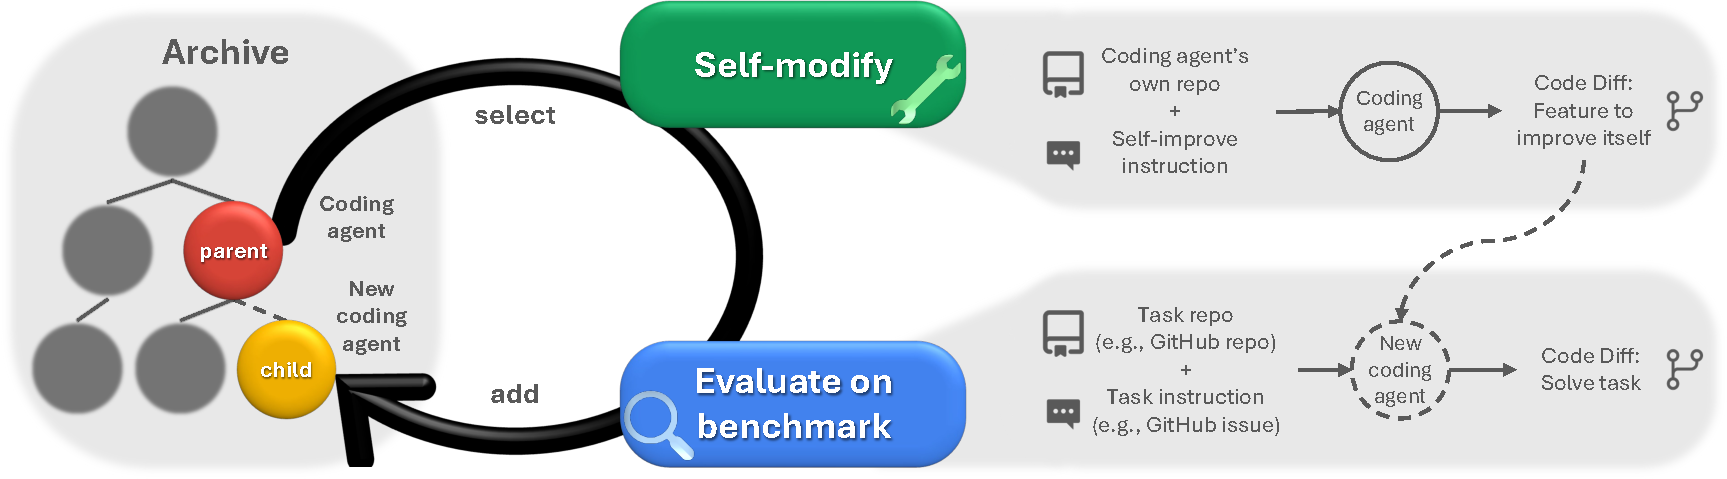
\includegraphics[width=.94\textwidth]{../papers/translations/dgm/figures/conceptual.pdf}
\caption{达尔文哥德尔机. DGM 交替执行自我修改与下游任务评价，迭代构建不断扩大的智能体档案. 通过开放式探索，选择档案中的智能体执行自我修改. 原图：Jenny Zhang、Shengran Hu、Cong Lu、Robert Lange、Jeff Clune，CC BY 4.0；图内英文标注保留.}\label{dgm-fig:conceptual}
\end{figure}

Schmidhuber\cite{dgm-schmidhuber2007godel}提出了一类具有严格数学基础的、自指的、自我改进问题求解器. 它依赖形式证明来论证代码重写，确保任何自我修改都可证明有益. 但在实践中，如果不对系统作限制性假设，就无法形式证明对人工智能系统的一项修改是否有益. 例如，看似给基于大语言模型的编码智能体更多工具——代码搜索、测试运行器等——会带来益处，但实际影响高度依赖模型训练和任务上下文；针对一种设置优化的测试工具，可能在另一种设置下让智能体困惑. 我们不要求形式证明，而是根据基准经验验证自我修改，使系统能依据观测结果改进和探索. 这类似生物演化：突变和适应并不事先得到验证，而是在产生、试验之后经自然选择保留. 我们也从达尔文演化\cite{dgm-darwin2023origin}获得启发，研究保留此前发现的智能体库、让其成为后代垫脚石的有效性.

我们提出\textbf{达尔文哥德尔机（DGM）}，一种自指、自我改进系统，通过编写和修改自己的代码成为更好的编码智能体. 每次自我修改都要求 DGM 编辑自己的代码库. 我们使用图灵完备的 Python，因此 DGM 在潜力上能够构建任何可计算机器. 我们的框架设想智能体可以重写自己的训练脚本，包括训练新的基础模型（FM）. 但本文没有展示这一点，因为训练基础模型计算量很大，会引入大量额外复杂性，我们将其留作未来工作. 本文聚焦于使用冻结预训练基础模型的编码智能体设计改进，如工具使用与工作流. DGM 交替执行自我修改和评价. 自我修改阶段，从档案中选出的编码智能体生成自己的修改版本；评价阶段，对每个修改后的智能体进行编码基准测试，估计其编码能力，再加入档案. 通过这一循环改善能力后，DGM 在解决编码任务和进行未来自我改进方面都变得更好. 一个关键假设是，编码基准表现提高意味着编码能力更好，从而自我修改与自我改进能力也更好. 此外，DGM 维护生成智能体的档案，从一个智能体开始，随时间持续积累全部变体. 为支持持续自我改进，DGM 借鉴开放式研究\cite{dgm-wang2019paired,dgm-fernandopromptbreeder,dgm-faldor2025omni}，积累多样的垫脚石，即有趣但次优、可能促成未来突破的解或特征. 开放式探索鼓励发现超出即时性能收益的新颖且可能有用的自我修改.

我们在两个编码基准 SWE-bench\cite{dgm-jimenez2024swebench}与 Polyglot\cite{dgm-gauthier2024polyglot}上报告结果. DGM 在 SWE-bench 上从 20.0\% 自动提高到 50.0\%，在 Polyglot 上从 14.2\% 提高到 30.7\%. 我们表明，自我改进支持持续进步：DGM 优于始终用同一个基础智能体修改并生成新智能体、却不进行自我改进的基线. 我们还表明，开放式探索与保留全部此前生成智能体的档案，有助于发现更好的编码智能体. DGM 优于不进行开放式探索的基线；后者不积累有趣且彼此不同的垫脚石档案，编码智能体始终建立在自身最新版本上. 总体而言，DGM 朝着能积累先前创新并递归改进的人工智能系统迈出了一步. 我们广泛讨论安全问题，包括沙箱化和自我修改的可追溯性，以保证负责任的实验（见\ref{dgm-sec:safety}节）. 推进安全、自指、自我改进模型的可能性，使我们更接近不仅会学习、还会像科学一样沿开放式、自加速轨迹演化的人工智能.

\originalsection{2 相关工作}\paperlabel{2}{dgm-sec:related}
\textbf{开放式.} 推动无界创新的一项重大挑战，是设计不断生成新颖且可学习成果的开放式人工智能系统\cite{dgm-stanley2017open}. Hughes 等\cite{dgm-hughes2024open}把开放式刻画为系统从观察者视角生成既新颖又可学习的成果序列的能力. 核心困难是如何组织和探索庞大搜索空间，持续产生对人有趣的成果\cite{dgm-clune2019ai,dgm-jiang2023general}. 早期进展来自质量多样性算法、目标导向探索、内在动机和学习进度框架\cite{dgm-pugh2016quality,dgm-ecoffet2019go,dgm-lehman2011novelty,dgm-oudeyer2007intrinsic}；近期进展则用大规模基础模型作为人类趣味的代理，并作为跨领域生成和评价新行为的通用引擎\cite{dgm-brown2020language,dgm-hu2025automated,dgm-zhang2024omni}. 但这些方法尚未闭合自指自我改进循环，即下游任务改进还未转化为更强的自我修改能力或进一步创新的加速. 我们希望模拟科学技术的加速过程，新工具和发现会催生更多发现. 如何模仿自然的演化轨迹，使其不仅朝复杂性发展，还朝着越来越强的演化能力发展\cite{dgm-dawkins2019evolution,dgm-gerhart2007theory,dgm-hendrikse2007evolvability}？

\textbf{基础模型智能体的元学习.} 许多基于基础模型的智能体由人工设计. 构建模块包括提示工程\cite{dgm-chen2023unleashing,dgm-schulhoff2024prompt}、思维链\cite{dgm-wei2022chain,dgm-yao2023react,dgm-hu2023ThoughtCloning,dgm-guo2025deepseek,dgm-lightman2023let,dgm-muennighoff2025s1,dgm-zelikman2024quiet}、自我反思\cite{dgm-shinn2023reflexion,dgm-yao2023react,dgm-madaan2303self}、多智能体辩论\cite{dgm-zhuge2023mindstorms,dgm-liang2023encouraging,dgm-khan2024debating}、记忆\cite{dgm-liu2023think,dgm-zhong2024memorybank,dgm-modarressi2023ret}、温度采样\cite{dgm-zhu2024hot}与检索增强生成\cite{dgm-lewis2020retrieval}. 人工组合这些模块，会让系统能力受限于设计者的创造力. 近期出现的元学习方法使用基础模型自动优化提示\cite{dgm-fernandopromptbreeder,dgm-meta2022human,dgm-khattab2023dspy,dgm-cheng2025trace,dgm-yuksekgonul2024textgrad,dgm-yuan2024evoagent}和设计智能体模块\cite{dgm-zhang2024aflow,dgm-zhou2024symbolic,dgm-yin2024g,dgm-zhugegptswarm,dgm-rosser2025agentbreeder,dgm-zhang2025multi,dgm-ye2025mas,dgm-gao2025flowreasoner,dgm-nie2025weak,dgm-su2025debflow,dgm-zhang2025gnns,dgm-niu2025flow}. 智能体系统的自动化设计（ADAS）\cite{dgm-hu2025automated}用固定的元智能体迭代生成下游智能体，在目标基准上评价，并利用反馈改进后续生成. 相比之下，DGM 是单一系统，既解决下游编码问题，又改进自己的实现即代码库，不再需要固定、人工设计的元智能体，从而支持自指改进.

\textbf{自我改进人工智能.} 早期研究者提出了自我改进的理论和概念方案\cite{dgm-good1966speculations,dgm-schmidhuber1987evolutionary,dgm-schmidhuber2007godel}. 一些实践方法包括以神经网络权重参数化定义的系统\cite{dgm-schmidhuber1993self,dgm-hall2007self,dgm-hobbhahn2025swebenchmini,dgm-kirsch2022self,dgm-irie2022modern,dgm-irie2025metalearning,dgm-lu2023arbitrary,dgm-havrilla2024glore}. Metz 等\cite{dgm-metz2021training}开发了一个基于梯度的优化器，利用种群训练\cite{dgm-jaderberg2017population}的变体进行自指元训练. Lange 等\cite{dgm-lange2023discovering}把这种方案扩展到无梯度学习. Silver 等\cite{dgm-silver2017mastering}利用自博弈持续演化智能体，在国际象棋与围棋等困难领域取得超人表现. 更接近 DGM 的是近期使用基础模型智能体进行自我改进的方案\cite{dgm-yin2024g,dgm-robeyns2025self,dgm-hu2024self,dgm-zelikman2024self,dgm-huang2022large,dgm-singh2023beyond}. Zelikman 等\cite{dgm-zelikman2024self}用元智能体生成下游智能体，再依据生成解的元效用更新元智能体. Yin 等\cite{dgm-yin2024g}用同一个系统解决下游任务并递归修改自身. 但下游任务或元效用并不总与自我改进所需能力一致. 在 DGM 中，下游任务提升直接反映自我改进能力增强，因此具有自加速进步的潜力. 最相似的同期工作是 Robeyns 等\cite{dgm-robeyns2025self}，它也让单一智能体递归解决编码问题并修改自己的代码库. 与该工作以及 Zelikman 等、Yin 等的主要区别在于，DGM 具有开放式探索循环，鼓励超越即时收益的自我修改，避免在次优状态停滞. 附录\hyperref[dgm-app:related]{B}还讨论程序合成与达尔文演化的相关工作.

\originalsection{3 达尔文哥德尔机}\paperlabel{3}{dgm-sec:methods}
哥德尔机是一种理论构想：寻找可证明能改进自身的方法的人工智能\cite{dgm-schmidhuber2007godel}. 本文提出 DGM，尝试实现创造哥德尔机的长期梦想. DGM 放宽了哥德尔机不切实际的要求，即从理论上证明一项变化能改善系统；它改为要求通过实验中的经验证据，展示所提议的新版本提升了表现. 此外，依赖改进的经验证据，可能让 DGM 陷入全部可计算算法这一庞大可能系统空间的局部最优. 为此，DGM 在搜索中维护已发现解的档案，支持开放式探索，而不只演化一个解. 这些原则呼应达尔文演化\cite{dgm-darwin2023origin}（附录\hyperref[dgm-app:related]{B}）：从此前发现解的档案选出实体、修改它，并在它以有趣方式变新时保留\cite{dgm-zhang2024omni,dgm-faldor2025omni,dgm-stanley2015greatness}. 因此我们把算法称为达尔文哥德尔机（图\ref{dgm-fig:conceptual}）.

\textbf{编码智能体的自指自我改进.} DGM 仅以一个编码智能体初始化，并用编码基准评价进展. 编码智能体定义为一个以代码仓库实现、由冻结预训练基础模型驱动、能读写和执行代码的单一系统. 用 Python 等通用图灵完备语言表达的代码，是构建与改进智能系统的强大媒介，因为它可以表示任何可计算过程. 近期工作\cite{dgm-hu2025automated,dgm-zhang2024aflow}表明，可以通过对代码仓库中实现的提示、工作流与工具等设计进行元学习来改进智能体. 因而，我们把自我改进定义为修改智能体自身模块设计、也就是自身代码的一项编码任务；不包含下一段的开放式探索过程. 关键动机在于，经验证据必须同时反映系统自我改进和解决下游任务的能力. 把 DGM 配置为编码智能体并测试编码能力，观察到的改进不仅展示下游表现增强，也展示进一步自我改进的能力，因为自我改进本质上是一项修改编码智能体自身代码仓库的编码任务.

\textbf{基于种群的开放式探索.} DGM 从一个初始编码智能体开始，建立全部已发现智能体的档案. 每次迭代选出父智能体，让其自我修改并分支产生新智能体. 父代选择大体正比于各智能体的表现分数，反比于具有代码库编辑功能的子代数（附录\hyperref[dgm-app:parent-select]{C.2}）. 这偏向表现良好而探索不足、即现有子代较少的智能体，兼顾利用强表现者与探索有希望但采样较少的谱系. 每个智能体保留非零选择概率，确保在计算资源足够时任何改进路径仍有可能. 每个被选父代分析自己的基准评价日志，提出下一项待实现功能，再把提案作为问题描述执行（附录\hyperref[dgm-app:selfimprove-prompts]{C.3}）. 父代将建议功能实现在自身代码库中，生成新编码智能体. 每个新智能体在选定编码基准上被定量评价，估计其编码能力. 只有成功编译且仍能编辑指定代码库的智能体才加入档案，因为只有它们能继续自我修改，其余均被丢弃. 父代选择、自我修改与评价循环不断进行，逐步扩充解的档案. 重要的是，归档的解可能成为在很久之后才带来改进的垫脚石，因此本方法与爬山式智能体设计\cite{dgm-robeyns2025self}有实质区别. 当前开放式探索过程，即档案维护与父代选择，是固定的，不能由 DGM 修改；我们将其留作未来方向. 附录\hyperref[dgm-app:pseudocode]{C.4}给出算法伪代码.

\originalsection{4 实验}\paperlabel{4}{dgm-sec:experiments}
第\ref{dgm-sec:experiment-setup}节介绍包括初始编码智能体在内的实验设置. 我们在 SWE-bench\cite{dgm-jimenez2024swebench}和 Polyglot\cite{dgm-gauthier2024polyglot}上实验（第\ref{dgm-sec:benchmarks}节）. 每个基准均比较 DGM 与两个基线：无自我改进智能体的 DGM、无开放式探索的 DGM（第\ref{dgm-sec:baselines}节）. 所有实验中 DGM 都优于两个基线，表明自我改进机制与开放式探索对持续性能增益至关重要（第\ref{dgm-sec:results}节）. 我们还展示所发现特征能跨模型、基准和任务迁移.

\originalsection{4.1 实验设置}\paperlabel{4.1}{dgm-sec:experiment-setup}
DGM 以单一编码智能体初始化. 基础智能体围绕冻结基础模型构建，增加工具使用能力\cite{dgm-schick2023toolformer,dgm-anthropic_tool_use_2024}. 基础模型自主决定每一步的动作，使用它认为适合的工具. 基础智能体有两个工具：执行 bash 命令的 Bash 工具，以及查看和编辑目录、整个文件的编辑工具（附录\hyperref[dgm-app:initial-agent]{C.1}）. 智能体收到一个输入提示，说明目标仓库位置、问题描述和仓库测试框架. 我们故意让基础智能体保持轻量，提供可清楚展示自我改进的简单起点. DGM 运行 80 次迭代，每次生成一个新智能体；SWE-bench 同时运行两次迭代，Polyglot 同时运行四次（附录\hyperref[dgm-app:parent-select]{C.2}）. 两个基准中的自我修改均由 Claude 3.5 Sonnet（New）\cite{dgm-anthropic2024claude35sonnet}驱动. 基准评价时，SWE-bench 使用 Claude 3.5 Sonnet（New），Polyglot 使用 o3-mini\cite{dgm-openai2025o3mini}（附录\hyperref[dgm-app:fm-hyperparam]{D.1}）.

\originalsection{4.2 基准}\paperlabel{4.2}{dgm-sec:benchmarks}
我们在两个流行编码基准上评价 DGM；它们考察编码任务的不同方面，从而验证算法在不同用例中的有效性. SWE-bench 与 Polyglot 均评价人工智能智能体自动解决编码任务的能力. 给定代码仓库和任务指令，智能体需修改仓库以完成任务. 二者均被广泛使用\cite{dgm-zhang2024autocoderover,dgm-zhang2024rest,dgm-xia2024agentless,dgm-cao2024spider2,dgm-GoogleDeepMind2025GeminiThinking,dgm-aider2024}，要求智能体浏览仓库、理解不同文件中函数的关联，在复杂代码里识别细小错误. SWE-bench 只有 Python 任务，Polyglot 涵盖多种语言. 另一个区别是，SWE-bench 任务可能需编辑多个文件，而 Polyglot 主要需在单个文件从头实现解法；尽管仍需查看其他文件来理解必要修改，但总体编辑文件数更少.

\textbf{SWE-bench.} 为避免在不可解任务上浪费计算，我们使用 SWE-bench Verified\cite{dgm-openai2024sweverified}，即经人工筛选、所有任务均可解的 SWE-bench\cite{dgm-jimenez2024swebench}子集. 本文的 SWE-bench 默认指这一 Verified 子集.

\textbf{Polyglot.} Polyglot 包含 C++、Rust、Python 等多种编程语言任务\cite{dgm-gauthier2024polyglot}. 相比最常用且可能已包含于基础模型训练集的 SWE-bench，Polyglot 更小众，更不可能包含于基础模型后训练数据. 此外，Polyglot 主要由其开发者用于评价 Aider\cite{dgm-aider2024}. 这提供了比较自动设计智能体与社区代表性编码智能体的机会，后者由人类开发者持续开发，并针对 Polyglot 测试超过一年. Polyglot 还允许检验 DGM 超出 Python、泛化到多语言的能力. 我们遵循 Polyglot 排行榜设置，但有一项关键区别：排行榜报告 pass@2，允许智能体查看一次真实测试反馈；我们报告 pass@1，智能体从不看到真实测试结果.

完整基准评价昂贵（附录\hyperref[dgm-app:cost-estimate]{E.1}），我们因此采用分阶段评价来估计编码表现. 一般而言，越确信某智能体相对强，就用更多任务评价它. 先在 10 项任务上验证基本代码库编辑功能. 只有仍能编辑代码的智能体，才可解决下游编码任务或继续自我修改. 通过初始阶段后，再在扩展的 50 项任务上评价. SWE-bench 任务依据 SWE-bench-verified-mini\cite{dgm-hobbhahn2025swebenchmini}选择，后者旨在代表完整基准（附录\hyperref[dgm-app:swebench-tasks]{E.2}）；Polyglot 任务为完整基准的随机子集（附录\hyperref[dgm-app:polyglot-tasks]{E.3}）. 所用大语言模型固有的随机性会造成表现噪声. 较小子集用于估计总体有效性、识别优良候选. SWE-bench 中，若智能体在 60 任务子集上成功率超过 40\%，且排在档案前两名，就再在 200 个任务上评价，即原 60 个加 140 个，以更精确衡量真实编码能力；40\% 是依据预运行噪声选择的启发式阈值. Polyglot 中，若在 10 任务子集上成功率超过 40\%，则在扩展的 50 任务子集上评价.

\originalsection{4.3 基线}\paperlabel{4.3}{dgm-sec:baselines}
为隔离 DGM 核心组件的贡献，我们比较\textbf{无自我改进的 DGM}与\textbf{无开放式探索的 DGM}. 前者在此设置下复现 ADAS\cite{dgm-hu2025automated}的方法：负责修改编码智能体的元智能体在整个实验中始终固定为基础智能体（原文算法 2）. 这用于考察迭代自我改进在加速更好编码智能体演化中的作用. 后者移除档案，始终修改最新保存的自身版本（原文算法 3）. 若智能体自我修改到丧失编辑代码库所需的基本功能，就无法继续修改自身或解决任何编码任务；因而该基线保留仍维持基本编辑功能的最新版本. 它用于评价档案以及已有充分记录的开放式探索有益原则\cite{dgm-clune2019ai,dgm-stanley2015greatness,dgm-zhang2024omni,dgm-fernandopromptbreeder,dgm-lee2020learning,dgm-samvelyan2024rainbow,dgm-colas2022autotelic}对智能体演化的作用.

除学习型基线外，我们还比较人工设计的开源方案. SWE-bench 采用经核验、即 SWE-bench 团队能复现结果的最佳开源方案（附录\hyperref[dgm-app:swebench-sota]{E.4}）. Polyglot 采用代表性智能体 Aider\cite{dgm-aider2024}，它开源且设计为支持多语言和大型代码库编辑（附录\hyperref[dgm-app:polyglot-sota]{E.5}）. 为公平比较，在评价 DGM 的相同任务子集上测量解题比例；图\ref{dgm-fig:dgm-comparisons}中的水平虚线展示这些值.

\originalsection{4.4 结果}\paperlabel{4.4}{dgm-sec:results}
\begin{figure}[ht]
\centering
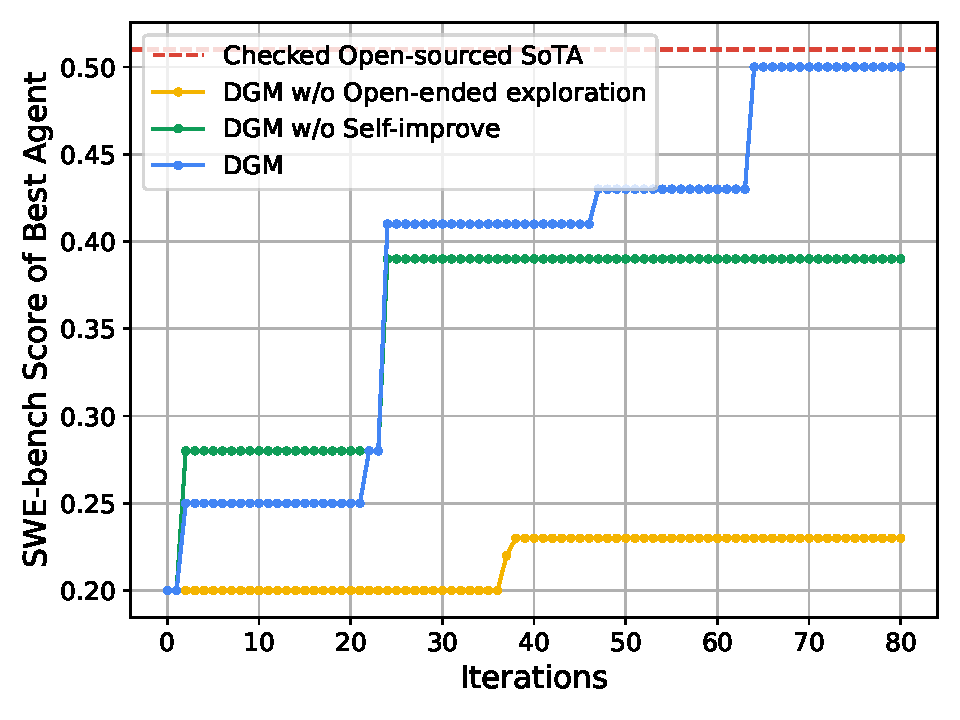
\includegraphics[width=.47\textwidth]{../papers/translations/dgm/figures/dgm_comparisons.pdf}\label{dgm-fig:dgm-comparisons-swe}
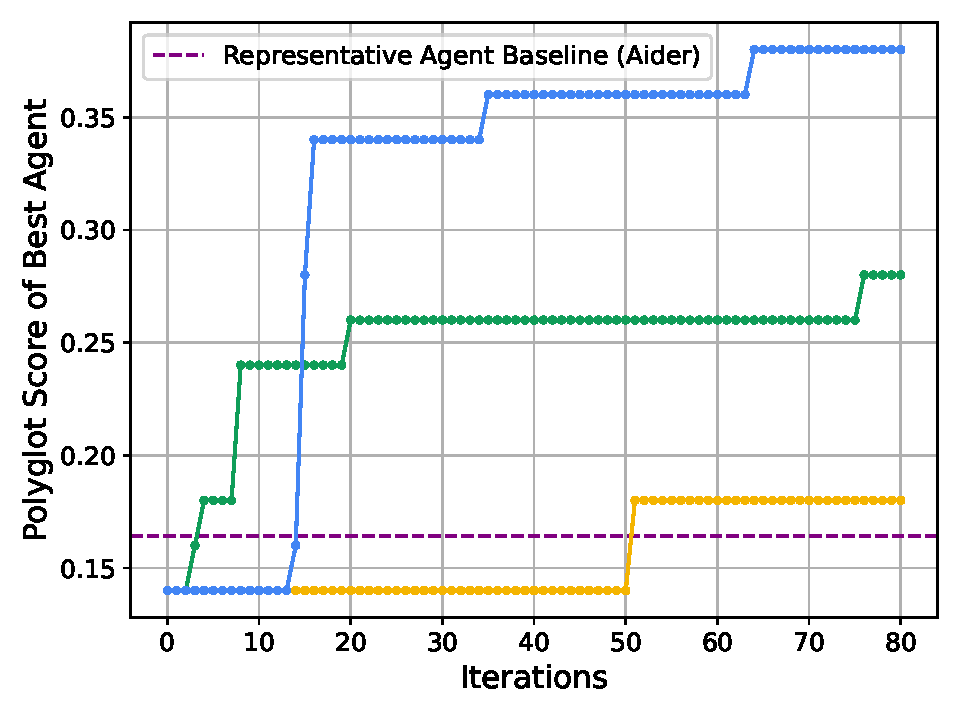
\includegraphics[width=.47\textwidth]{../papers/translations/dgm/figures/dgm_comparisons_polyglot.pdf}\label{dgm-fig:dgm-comparisons-polyglot}
\caption{自我改进与开放式探索使 DGM 持续进步并改善表现. DGM 自动发现越来越好的编码智能体，在左侧 SWE-bench 与右侧 Polyglot 上均取得更好表现. 它优于缺少自我改进或开放式探索的基线，表明两个组件对持续自我改进都至关重要. 分数来自第\ref{dgm-sec:benchmarks}节所述基准子集. 原图：Jenny Zhang、Shengran Hu、Cong Lu、Robert Lange、Jeff Clune，CC BY 4.0；英文标注保留.}\label{dgm-fig:dgm-comparisons}
\end{figure}
\begin{figure}[ht]
\centering
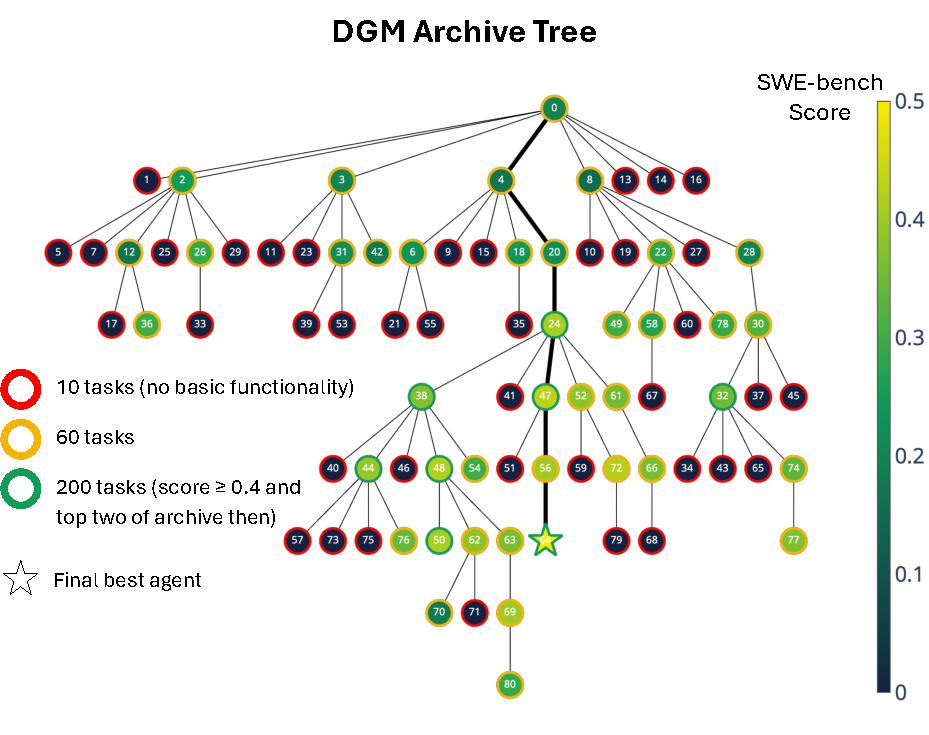
\includegraphics[width=.47\textwidth]{../papers/translations/dgm/figures/dgm_archive.pdf}
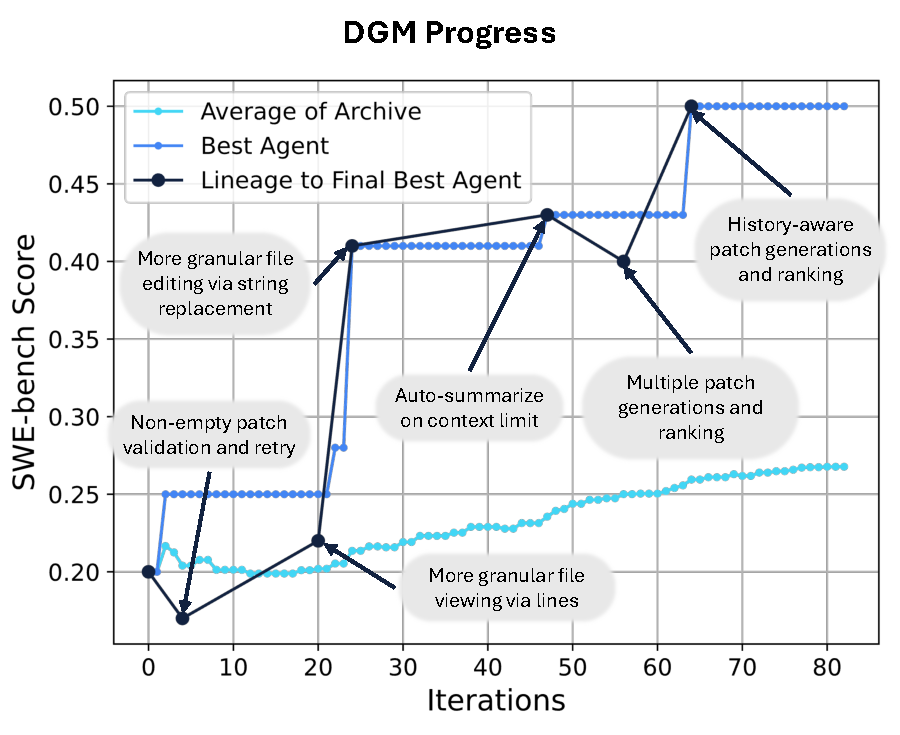
\includegraphics[width=.47\textwidth]{../papers/translations/dgm/figures/dgm_progress.pdf}
\caption{DGM 自动自我改进，成为更好的编码智能体. 左：SWE-bench 运行中生成的智能体档案. 每个节点代表一个编码智能体，节点 0 是基础智能体. 节点颜色表示 SWE-bench 表现即解题百分比，边框颜色表示该智能体评价过的任务数. 边表示哪个智能体自我修改产生了子代. 许多创新路径经过表现较差的节点，而节点 24 等关键创新引发建立于其上的创新爆发；这两点都体现开放式搜索的益处. 右：SWE-bench 上的 DGM 进展图. 浅蓝线是全部具有基本代码库编辑功能智能体的平均分，蓝线是每次迭代时档案中任一智能体达到的最高分，深色线是最终最佳智能体及其前驱的谱系，其中有两次性能下降. 这展示开放式搜索的益处：探索多样且有趣的垫脚石，而非只从当前最好解分支. 原图：Jenny Zhang、Shengran Hu、Cong Lu、Robert Lange、Jeff Clune，CC BY 4.0；英文标注保留.}\label{dgm-fig:dgm-archive}\label{dgm-fig:dgm-progress}
\end{figure}

80 次迭代后，编码智能体在 SWE-bench 上从 20.0\% 提高到 50.0\%，在 Polyglot 上从 14.0\% 提高到 38.0\%（图\ref{dgm-fig:dgm-comparisons}）. 因 Polyglot 实验设置仅评价 50 项任务，我们另在完整 Polyglot 基准上评价基础智能体和 DGM 发现的最佳智能体，以更精确估计改进；完整基准上从 14.2\% 提高到 30.7\%. 这表明 DGM 能自动自我改进，生成更好的编码智能体. 此外，所发现最佳智能体的表现可比于 SWE-bench 经核验、开源、人工设计的最佳方案. Polyglot 中，尽管基础智能体表现低于 Aider，DGM 仍发现了远超 Aider 的智能体. 两个基准中，发现的智能体可比于或优于人工设计智能体. SWE-bench 最佳智能体与 Aider 都经过人类精心塑造，而 DGM 提示了这样的未来：这种创造力可以自动化，通过持续自我改进的自指循环不断演化.

DGM 自动改善工具与基础模型的使用工作流（图\ref{dgm-fig:dgm-progress}）. 例如，它把编辑工具改为支持按行查看文件、通过字符串替换精确编辑，而非总是查看或替换整个文件. 工作流改进包括多次尝试解题，用另一基础模型评价并选出最好方案，以及生成后续尝试时考虑此前尝试. 附录\hyperref[dgm-app:best-agent-dgm]{F.1}与\hyperref[dgm-app:best-agent-dgm-polyglot]{F.2}分别展示通往两个基准最终最佳智能体的全部修改.

开放式探索允许以非零概率从档案中任何智能体分支，因此 DGM 能摆脱具有误导性的性能低谷或高峰. 例如 SWE-bench 的第 4 与 56 次迭代中，虽然智能体分数暂时低于父代，DGM 仍沿该路径探索创新，产生超过全部前驱的新智能体. 此外，开放式探索允许尝试相同目标功能的不同实现. 例如，更精细编辑工具的具体实现可以有很大差异，导致显著不同的表现（附录\hyperref[dgm-app:supp-dgm-diffimpl]{G}）. DGM 可以探索多个实现，寻找更适合的方案，而不陷入次优实现.

DGM 在两个基准上均优于无自我改进和无开放式探索的基线. 不更新负责修改编码智能体的元智能体时，无自我改进基线在初期提升智能体，但增益很快趋缓（附录\hyperref[dgm-app:plots-swe]{A.1}）. 无开放式探索基线只保留最近的智能体，因此表现差的自我修改会增加后续改进难度.

\begin{figure}[ht]
\centering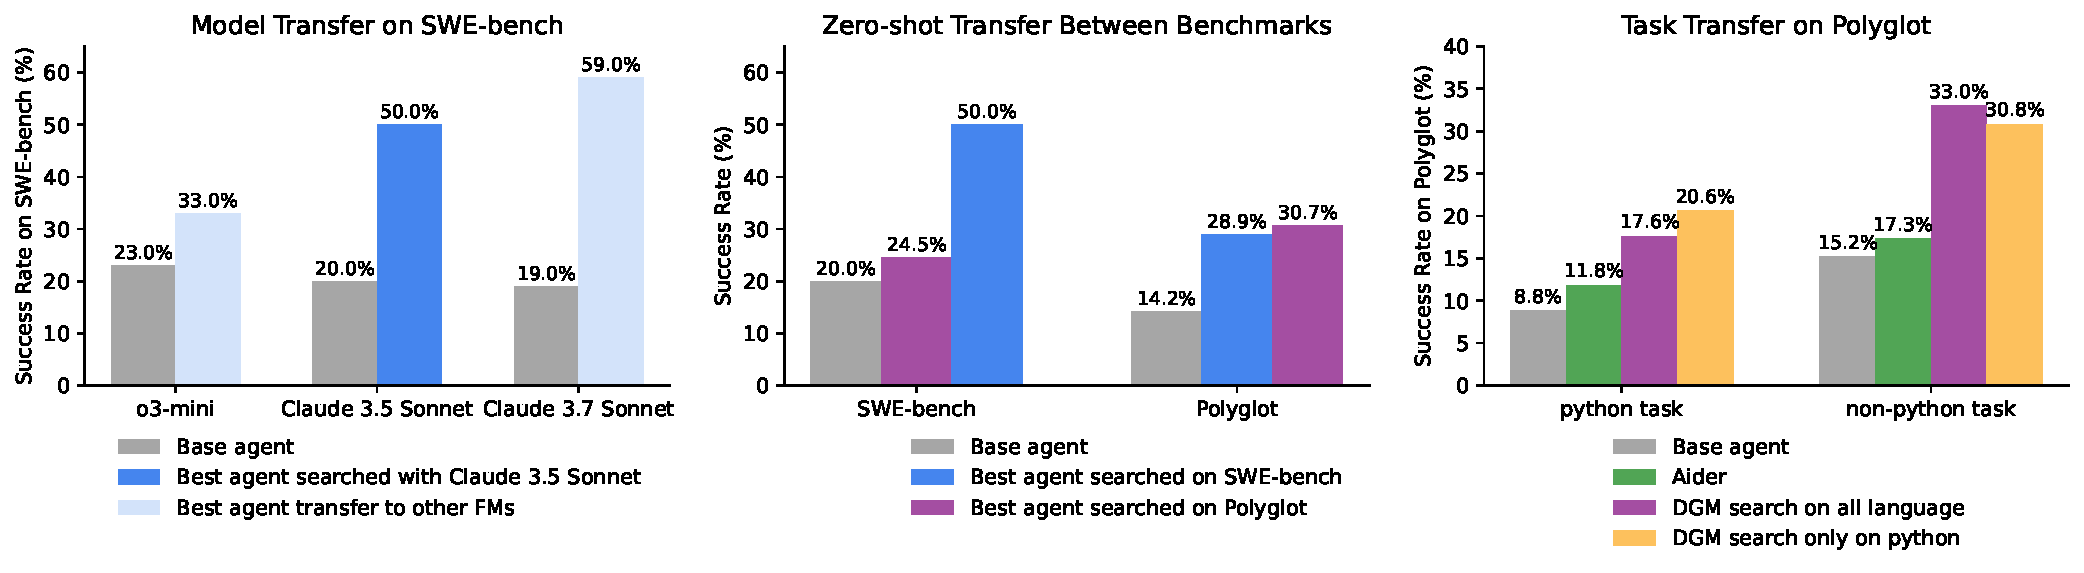
\includegraphics[width=.94\textwidth]{../papers/translations/dgm/figures/transfer_model_task.pdf}
\caption{模型、基准与任务间的迁移. DGM 发现智能体的更好表现可以迁移到不同模型（左）、不同基准（中），以及 Polyglot 中不同编程语言的任务（右），例如从 Python 任务迁移到 C++ 任务. 原图：Jenny Zhang、Shengran Hu、Cong Lu、Robert Lange、Jeff Clune，CC BY 4.0；英文标注保留.}\label{dgm-fig:transfer-overview}
\end{figure}

为评价改进的普遍性，我们用不同于优化时使用的基础模型测试基础智能体与运行中发现的最佳智能体. SWE-bench 运行使用 Claude 3.5 Sonnet（New），迁移评价把模型替换为 Claude 3.7 Sonnet\cite{dgm-anthropic2025claude37}或 o3-mini，在 200 个任务上评价（图\ref{dgm-fig:transfer-overview}左）. 使用 o3-mini 时，基础智能体 23.0\%，发现智能体 33.0\%；使用 Claude 3.7 Sonnet 时，分别为 19.0\% 与 59.5\%. 这提示改进可跨基础模型泛化，而非紧密耦合于运行时使用的特定模型. Polyglot 模型迁移结果见附录\hyperref[dgm-app:polyglot-model]{A.2}.

我们进一步研究跨基准和编程语言迁移. 首先，把在一个基准如 SWE-bench 上发现的最佳智能体用于完全留出的另一基准如 Polyglot，反向亦然（图\ref{dgm-fig:transfer-overview}中）. SWE-bench 演化出的最佳智能体在 Polyglot 达到 28.9\%，初始基线是 14.2\%；Polyglot 演化出的最佳智能体在 SWE-bench 达到 24.5\%，原基线是 20.0\%. 每个智能体优化时从未访问另一基准，因此这些评价是真正的留出测试. 跨基准一致的增益支持我们关于改进反映通用技能获得、而非过拟合或利用基准特定痕迹的论断. 其次，我们用只在 Polyglot 的 Python 任务上训练的 DGM，再把发现智能体迁移到其他语言. 与全语言训练相比，聚焦 Python 稍微改善 Python 表现，但降低非 Python 表现（图右）. 然而，从 Python 迁移到搜索时未见的语言后，智能体仍达到可比于全语言 DGM 的表现，显著优于基础智能体与 Aider. 这些结果展示改进的稳健性，说明并未过拟合于某一语言. 附录\hyperref[dgm-app:add-results]{A}给出更多结果.

\originalsection{5 安全讨论}\paperlabel{5}{dgm-sec:safety}
DGM 等自我改进系统朝更自主的人工智能开发迈出一步，符合构建能造福人类的强人工智能这一长期目标\cite{dgm-schmidhuber1987evolutionary,dgm-clune2019ai,dgm-markoff2016machines,dgm-lehman2023machine}. 但自主修改自身代码的能力带来独特安全问题. 即便提高目标指标，只针对基准优化的修改也可能意外引入漏洞或偏离人类意图的行为\cite{dgm-bostrom2020ethical}. 尤其当评价基准不能完整刻画安全和稳健等期望属性时，自我改进循环可能在连续世代中放大不对齐. 迭代自我修改还可能导致日益复杂、难解释的内部逻辑，妨碍理解、监督和控制\cite{dgm-sheth2025safety,dgm-anwar2024foundational,dgm-greenblatt2024alignment,dgm-ganguli2022red}.

针对这些挑战，当前实现与实验有若干防护. 所有智能体执行和自我修改都在隔离沙箱中进行，限制对宿主系统的影响，降低非预期行动风险. 每次沙箱执行有严格时限，减少资源耗尽和无界行为风险. 自我改进当前限于通过修改自己的 Python 代码库来提高特定编码基准表现这一明确领域，限制修改范围. 此外，我们主动监测表现与代码变化，档案提供可追溯的修改谱系以供审查. 目前未发现生成智能体具有有害或恶意行为的证据，自我修改主要聚焦提高编码能力.

反过来，自我改进范式的一项潜在重要益处，是原则上可以用于加强安全和可解释性本身. 我们初步研究如何在人工智能安全场景部署 DGM，开发应对基础模型幻觉的方法（附录\hyperref[dgm-app:dgm-halluc]{H}）. 如同学习改进编码能力，如果评价标准包含相应属性\cite{dgm-rosser2025agentbreeder}，DGM 可能发现并整合更好的内部防护，或通过修改提高透明度，如纳入类似 Constitutional AI 的原则\cite{dgm-bai2022constitutional}. 这提示一条有希望但具挑战的路径：把自我改进用作构建更可信人工智能的工具. 还可研究从一开始引入 Constitutional AI；困难是如何激励系统保留这些准则. 值得探索的一种方案是设置不可修改的系统部分，用于评价并停止其余部分.

由于当前前沿基础模型能力限制以及沙箱等有效缓解措施，DGM 在保持安全研究边界的同时展示自我改进潜力. 附录\hyperref[dgm-app:safety]{I}进一步讨论更广的安全不确定性. 我们主动加入安全讨论，以提高对自我改进系统新兴前景及相关安全影响的认识，尤其考虑到它们必然会更有能力\cite{dgm-yudkowsky2008artificial,dgm-bostrom2002a,dgm-ecoffet2020open,dgm-bengio2024managing,dgm-clune2019ai}. 因此，我们倡导继续研究生成人工智能的算法\cite{dgm-clune2019ai}与自我改进系统的安全、有益演化.

\originalsection{6 结论与局限}\paperlabel{6}{dgm-sec:conclusion}
我们提出 DGM，这是首个由基础模型驱动、具有开放式探索的自我改进系统，评价基准上的进步可以直接转化为更好的自我改进能力. 我们展示了自动发现更好的工具和基础模型系统，从而提高 SWE-bench 与 Polyglot 表现. 通过自我改进和开放式探索，DGM 表现持续上升，使我们向自加速、自我改进系统更进一步.

DGM 能自主达到与公开可用方案相当的表现，但仍不及 SWE-bench 最佳闭源方案. 运行更久是否持续产生收益并最终超过闭源方案，仍是开放问题. 闭源方案常依赖专家团队精心手工设计的技术. 基础模型在推理等能力上尚未达到这些专家水平，所以 DGM 当前需要大量计算来发现改进. 第\ref{dgm-sec:experiments}节所展示的一次 SWE-bench 运行约需两周，并产生可观 API 成本（附录\hyperref[dgm-app:cost-estimate]{E.1}）. 我们假设进一步进展需更高效利用计算资源并发展更好的推理能力.

本版本主要由基础模型驱动，因此固有地受其能力限制. 一项令人期待的未来方向是，把自我修改从提示和工作流扩展到计算需求更大的方法，如重写训练脚本、更新基础模型本身. 当前聚焦编码，而人工智能越来越广泛地应用于计算机视觉、创意写作等领域；另一个有希望的扩展是构建能在编码之外改进自身的系统. 本研究的关键假设是编码基准能良好反映自我改进能力，因为自我修改要求编辑自身代码库. 也可设想共同演化目标任务分布\cite{dgm-faldor2025omni,dgm-wang2023robogen}，像真正开放式过程一样，移除自我改进绑定单一目标的约束. 附录\hyperref[dgm-app:future-work]{J}列出更多方向. 继续探索这种强大技术时，必须如第\ref{dgm-sec:safety}节所述，把安全放在中心.

总之，DGM 通过能够编辑自身代码库的自我改进系统，朝人工智能开发自动化迈出了重要一步. 计算与推理限制当前约束了完整潜力，但基础模型与基础设施的持续进步可能释放更强、更通用的自我改进. 若能谨慎处理安全问题，自我改进系统与人工智能生成算法\cite{dgm-clune2019ai}的未来有巨大潜力，通过开放式演化不断重写或重新训练自身，追求与人类价值一致的更强能力.

\originalsection{伦理声明}\label{dgm-ethics}
我们确认遵守 ICLR 伦理守则. 本研究在代码编辑智能体这一有限背景下研究自我改进系统，并在标准编程基准上评价. 没有人类受试者，也未收集或处理个人身份信息，因此无需机构伦理审查委员会批准.

\textbf{安全与误用.} 若允许无约束行动，或优化意外引入不安全行为，自我修改系统可能构成安全风险. 所有实验智能体都在隔离沙箱中运行，有严格资源和时限；网络访问受限，不能修改宿主环境. 自我改进范围限于智能体自身 Python 代码库和评价框架. 我们维护完整可审计的代码修改与评价谱系，支持回滚与事后分析. 发现的智能体未部署于真实开发环境. 代码、提示和评价成果的发布计划将排除提升系统访问权限的组件，包含默认沙箱、防护与清楚的预期用途文档.

\textbf{两用性、下游影响与局限.} 更强自主编码智能体可能有两用性，如帮助软件维护，也可能在误用时帮助创建有害代码. 我们认为推进可控、可审计自我改进方法与展示实用防护的研究收益超过风险. 但明确不鼓励安全敏感或无沙箱部署，并提供具体安全建议（第\ref{dgm-sec:safety}节）. 对基准优化的经验关注可能不能覆盖稳健、可解释和广泛社会价值等全部属性. 因而我们把基准增益视为通用人工智能发展的必要但不充分指标，并讨论把安全、推理等目标纳入优化循环的路径.

\textbf{数据治理、知识产权与许可.} SWE-bench Verified 与 Polyglot 由开源仓库与任务构成. 据我们所知，实验遵守了数据集许可和使用条款. 我们没有引入或分发专有代码. 基础模型通过提供者 API、依其服务条款访问；没有提交敏感数据，也没有尝试绕过使用政策. 发布日志将清除 API 密钥及意外出现的敏感字符串.

\textbf{偏见、公平与平等.} 虽然领域是软件代码而非以人为中心的文本，基础模型行为仍可能反映语言或生态系统偏好等偏见，对训练数据中工具覆盖更好的社区带来不均衡收益. 我们通过 Polyglot 多语言评价与跨基准迁移报告部分应对此问题. 未来应诊断有偏失败模式，并纳入更广、由社区推动的任务集.

\textbf{利益冲突与资助.} 作者均无在本文评价产品中的财务利益. 除薪酬或常规研究支持外，资助者与雇主未影响实验设计、分析或发表决定. 外部计算资源或 API 额度在附录中致谢.

\originalsection{可复现性声明}\label{dgm-reproducibility}
我们将开源全部代码与完整智能体日志，包括自我修改的完整档案谱系、差异补丁、提示、配置和评价框架. 为支持精确复现，本文提供算法细节与伪代码（第\ref{dgm-sec:methods}节、附录\hyperref[dgm-app:pseudocode]{C.4}）、父代选择和开放式探索设置（附录\hyperref[dgm-app:parent-select]{C.2}）、基础模型选择与超参数（附录\hyperref[dgm-app:fm-hyperparam]{D.1}）、两个基准的任务子集（附录\hyperref[dgm-app:swebench-tasks]{E.2}、\hyperref[dgm-app:polyglot-tasks]{E.3}）、分阶段评价协议与脚本（第\ref{dgm-sec:benchmarks}节）、最佳发现智能体的实现与补丁（附录\hyperref[dgm-app:best-agent-dgm]{F.1}、\hyperref[dgm-app:best-agent-dgm-polyglot]{F.2}），以及计算与费用估计（附录\hyperref[dgm-app:cost-estimate]{E.1}）. 发布的代码仓库将包含环境规范以及复现全部结果、图与表的脚本.

\originalsection{致谢}\label{dgm-acknowledgments}
本研究得到 Vector Institute、Canada CIFAR AI Chairs 项目、Schmidt Futures 资助、NSERC Discovery Grant，以及 Rafael Cosman 的慷慨捐赠支持. 安大略省、加拿大政府通过 CIFAR，以及 Vector Institute 的赞助企业部分提供了研究准备所需资源（\url{https://vectorinstitute.ai/partnerships/current-partners/}）. 本材料表达的意见、发现、结论或建议均属于作者，并不必然反映资助者观点. 我们还感谢 Aaron Dharna、Ben Norman、Cédric Colas、Sam Devlin 和 Shyam Sudhakaran 的深入讨论和反馈.

\originalsection{附录目录}\label{dgm-appendix-contents}
原文附录依次为：A 补充结果，B 补充相关工作，C 算法细节，D 实验细节，E 基准细节，F 发现的最佳智能体，G 相似目标功能的不同实现，H 解决幻觉的案例研究，I 补充安全讨论，J 补充未来工作方向. 原文的自动目录在译稿中改为这一索引，全部实质内容按原顺序保留.

\originalsection{附录 A 补充结果}\paperlabel{A}{dgm-app:add-results}
\noindent\textbf{A.1 SWE-bench 上的基线}\phantomsection\label{dgm-app:plots-swe}\par
\begin{figure}[ht]
\centering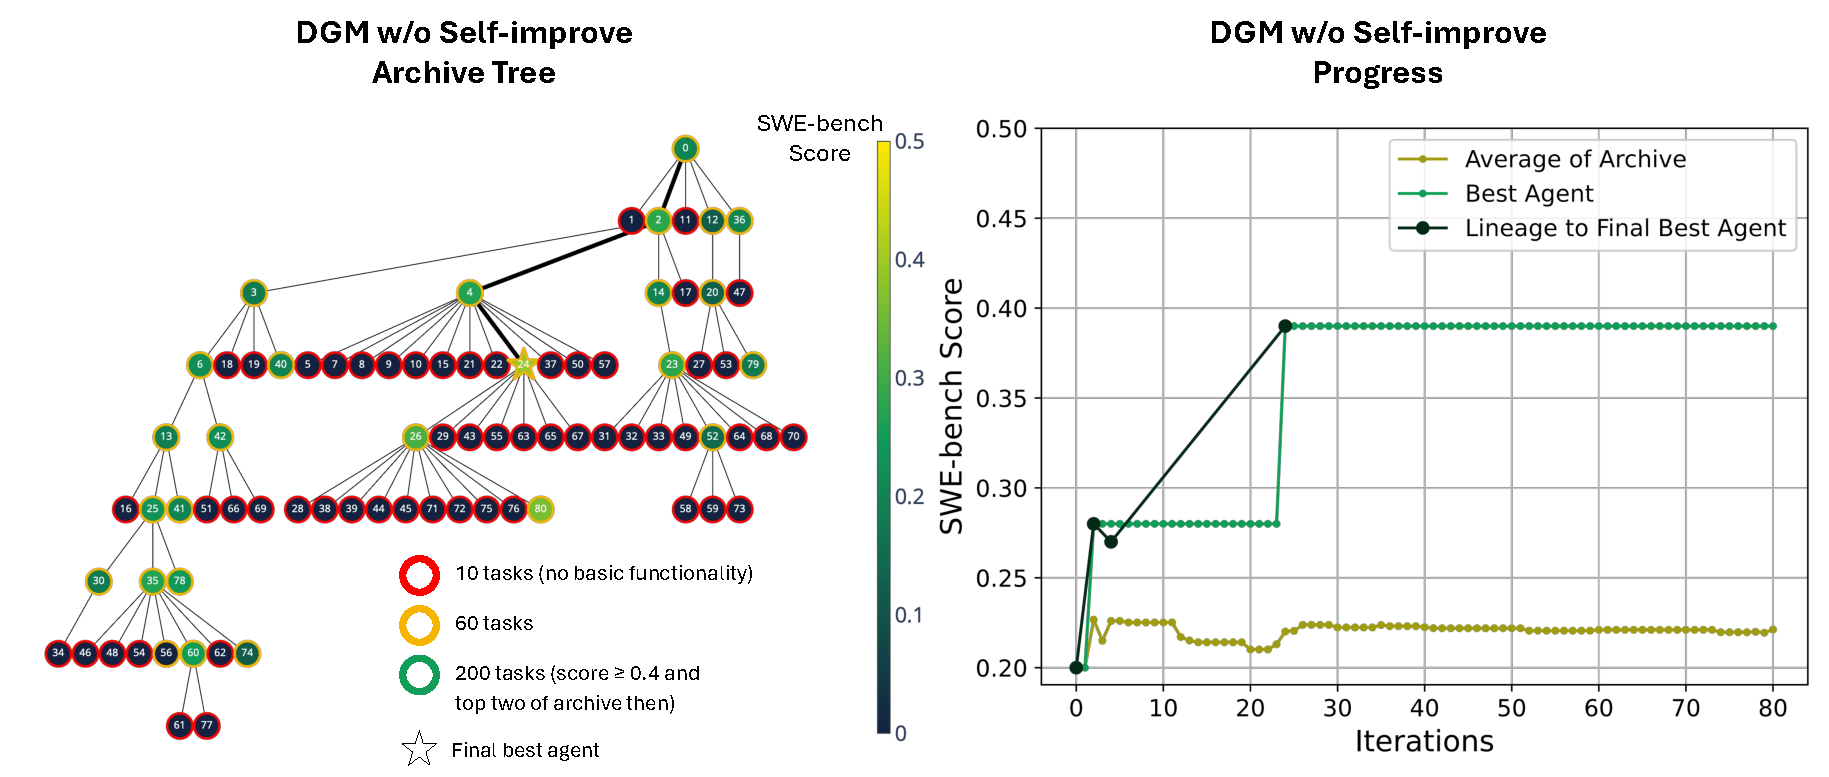
\includegraphics[width=.94\textwidth]{../papers/translations/dgm/figures/dgm_wo_selfimprove.pdf}
\caption{没有自我改进智能体的 DGM. 修改并生成下一代编码智能体的元智能体始终相同，因此该基线不能随时间持续改进. 左：SWE-bench 运行生成的编码智能体档案. 每个节点代表一个智能体，节点 0 是基础智能体；节点颜色表示 SWE-bench 解题百分比，边框颜色表示评价任务数，边表示哪个智能体自我修改产生子代. 右：SWE-bench 上该基线的进展图. 浅绿线是具有基本代码库编辑功能智能体的平均分，绿线跟踪每次迭代时档案中任一智能体达到的最高分，深色线是最终最佳智能体及其前驱的谱系. 原图：Jenny Zhang、Shengran Hu、Cong Lu、Robert Lange、Jeff Clune，CC BY 4.0；英文标注保留.}\label{dgm-fig:dgm-no-selfimprove}
\end{figure}
\begin{figure}[ht]
\centering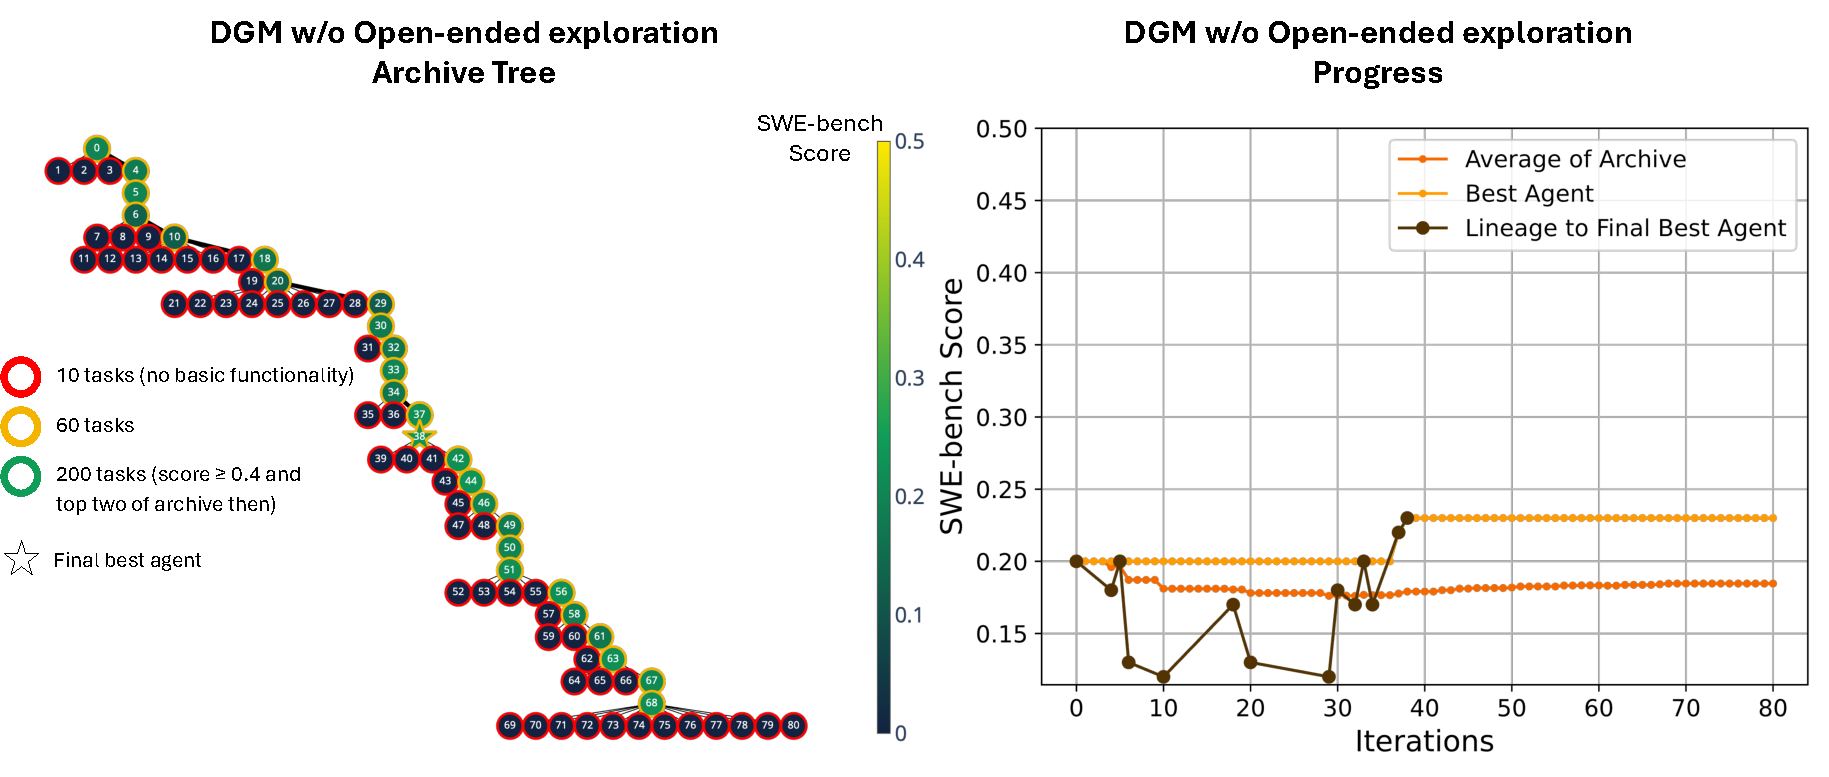
\includegraphics[width=.94\textwidth]{../papers/translations/dgm/figures/dgm_wo_openended.pdf}
\caption{没有开放式探索的 DGM. 移除档案后，该基线始终使用最近的智能体自我修改，在 SWE-bench 上进展很少. 左：运行中生成的智能体档案. 每个节点代表智能体，节点 0 是基础智能体；节点颜色表示解题百分比，边框颜色表示评价任务数，边表示父代自我修改生成子代. 右：进展图. 橙线是具有基本代码库编辑功能智能体的平均分，浅橙线跟踪每次迭代时档案中任一智能体达到的最高分，深色线是最终最佳智能体及其前驱谱系. 原图：Jenny Zhang、Shengran Hu、Cong Lu、Robert Lange、Jeff Clune，CC BY 4.0；英文标注保留.}\label{dgm-fig:dgm-no-openended}
\end{figure}

\noindent\textbf{A.2 Polyglot 上的跨模型普遍性}\phantomsection\label{dgm-app:polyglot-model}\par
\begin{figure}[ht]
\centering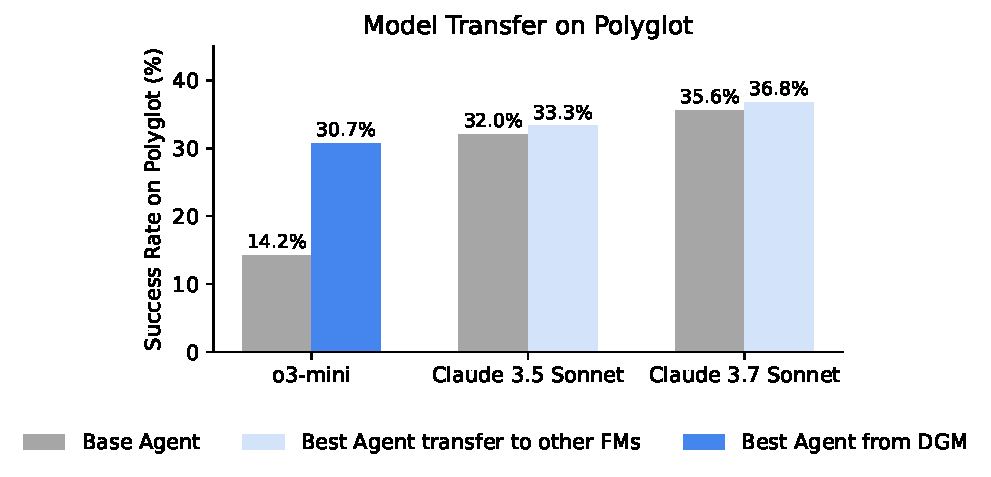
\includegraphics[width=.62\textwidth]{../papers/translations/dgm/figures/transfer_model_polyglot.pdf}
\caption{Polyglot 上的模型间迁移. 原图：Jenny Zhang、Shengran Hu、Cong Lu、Robert Lange、Jeff Clune，CC BY 4.0；英文标注保留.}\label{dgm-fig:transfer-model-polyglot}
\end{figure}
除 SWE-bench 上的模型迁移测试（第\ref{dgm-sec:results}节、图\ref{dgm-fig:dgm-comparisons}）外，本节报告 Polyglot 的迁移结果. Polyglot 的 DGM 运行使用 o3-mini；我们将基础模型替换为 Claude 3.5 Sonnet（New）或 Claude 3.7 Sonnet，并在完整基准上评价（图\ref{dgm-fig:transfer-overview}中）. Claude 3.5 Sonnet（New）下，初始智能体为 32.0\%，发现智能体为 33.3\%；Claude 3.7 Sonnet 下分别为 35.6\% 与 36.8\%. 这些结果提示 DGM 产生的改进可跨基础模型泛化，而非紧密绑定于运行时所用的特定模型.

\noindent\textbf{A.3 父代选择的消融}\phantomsection\label{dgm-app:parent-ablation}\par
为进一步研究父代选择机制，我们引入 DGM Greedy. 它总是选择表现最好的节点作为分支父代，而非像本实现一样让每个节点都有非零分支概率，其大小大致由表现分数和子代数决定（附录\hyperref[dgm-app:parent-select]{C.2}）. 该消融在此设置下复现 Robeyns 等\cite{dgm-robeyns2025self}的方法. 表\ref{dgm-tab:DGM-greedy}中，DGM Greedy 在 SWE-bench 与 Polyglot 分别达到 39.7\% 和 30.0\%，本实现则为 50.0\% 和 38.0\%. 这表明让档案中所有解都能成为潜在垫脚石，可以随时间带来更大改进，强调了开放式探索的重要性.
\begin{table}[ht]
\centering\caption{DGM、消融与基线在 SWE-bench 和 Polyglot 上的比较.}\label{dgm-tab:DGM-greedy}
\begin{tabular}{lcc}\toprule
方法&SWE-bench&Polyglot\\\midrule
DGM&50.0\%&38.0\%\\
无开放式探索&23.0\%&14.0\%\\
无自我改进&39.0\%&28.0\%\\
DGM Greedy&39.7\%&30.0\%\\\bottomrule
\end{tabular}
\end{table}

\noindent\textbf{A.4 DGM 运行的补充统计}\phantomsection\label{dgm-app:additional-statistics}\par
\textbf{生成智能体中具备基本代码编辑功能的比例.} 为更深入理解 DGM 过程，我们分析 SWE-bench 上生成智能体具有基本编辑功能的比例. 表\ref{dgm-tab:code_editing}显示 DGM 的比例最高. 结果突出开放式探索与自我改进的有效性：前者让搜索逃离局部最优，后者增强生成更好智能体的能力.
\begin{table}[ht]
\centering\caption{SWE-bench 上生成智能体具备基本代码编辑功能的比例.}\label{dgm-tab:code_editing}
\begin{tabular}{lc}\toprule 方法&比例\\\midrule
DGM&51.3\%\\无开放式探索&32.5\%\\无自我改进&32.5\%\\\bottomrule\end{tabular}
\end{table}
\textbf{DGM 运行的稳定性.} 为评价稳定性，我们在 Polyglot 上运行算法三次，分析性能方差. DGM 的平均准确率为 40.7\%，标准差为 2.3\%，表明它能在不同运行间取得一致且可复现的结果.

\originalsection{附录 B 补充相关工作}\paperlabel{B}{dgm-app:related}
\textbf{开放式（第二部分）.} 早期方法探索平衡可学习性与趣味性的不同机制. 质量多样性算法试图以多样的高表现行为照亮庞大解空间\cite{dgm-pugh2016quality,dgm-chatzilygeroudis2021quality,dgm-mouret2015illuminating,dgm-nguyen2015innovation}. 其他方法强调目标导向探索\cite{dgm-ecoffet2019go,dgm-ecoffet2021first,dgm-schaul2015universal,dgm-andrychowicz2017hindsight,dgm-eysenbach2018diversity}、内在动机\cite{dgm-lehman2011novelty,dgm-oudeyer2007intrinsic,dgm-li2014encouraging,dgm-pathak2017curiosity}或学习进度框架\cite{dgm-kanitscheider2021multi,dgm-gaven2025magellan,dgm-baranes2013active,dgm-colas2019curious,dgm-colas2022autotelic,dgm-jiang2021prioritized,dgm-dennis2020emergent,dgm-schmidhuber2008driven,dgm-schmidhuber2013powerplay,dgm-kompella2017continual}. 近期，大规模基础模型\cite{dgm-brown2020language,dgm-radford2019language}成为人类趣味概念的强代理\cite{dgm-zhang2024omni,dgm-faldor2025omni,dgm-sancaktar2025sensei}，也成为提出新代码解的有效突变算子\cite{dgm-romera2024mathematical,dgm-Novikov2025AlphaEvolve,dgm-lehman2023evolution,dgm-faldor2025omni,dgm-hu2025automated}. 基础模型可以引导自主设定目标的智能体\cite{dgm-colas2022autotelic,dgm-colas2023augmenting,dgm-colas2022language}，建模人类对质量和多样性的偏好\cite{dgm-bradley2023quality,dgm-ding2023quality,dgm-wang2023diversity,dgm-klissarov2023motif,dgm-klissarov2024maestromotif,dgm-samvelyan2024rainbow,dgm-lim2024large,dgm-havrilla2024surveying}，设计奖励函数\cite{dgm-wiering1997hq,dgm-wang2023voyager,dgm-ma2023eureka,dgm-faldor2025omni}，创建模拟环境\cite{dgm-sudhakaran2023mariogpt,dgm-nasir2023practical,dgm-aki2024llm,dgm-nasir2024word2world,dgm-bruce2024genie,dgm-parkerholder2024genie2,dgm-schmidhuber2013powerplay}，驱动不断演化的多智能体动态\cite{dgm-dharna2024quality,dgm-zhou2025autoredteamer}，搜索多样的行走机器人形态\cite{dgm-lehman2023evolution}，并为基准或目标优化搜索广阔解空间\cite{dgm-lange2024large,dgm-zhang2024omni,dgm-faldor2025omni,dgm-hu2025automated,dgm-lu2024intelligent,dgm-romera2024mathematical,dgm-fernandopromptbreeder,dgm-lu2024ai,dgm-khan2024debating,dgm-lu2025automated,dgm-liu2024evolution,dgm-Novikov2025AlphaEvolve}.

\textbf{程序合成.} 程序合成\cite{dgm-alur2018search,dgm-polozov2015flashmeta,dgm-buchi1990solving,dgm-gulwani2011automating,dgm-ellis2021dreamcoder}旨在生成符合输入输出样例或逻辑公式等外部规范的代码. 混合方法把符号方法与神经网络或基础模型引导结合：Li 等\cite{dgm-li2024guiding}用大语言模型建议引导 SyGuS 场景中的符号搜索，优于纯枚举；Barke 等\cite{dgm-barke2024hysynth}结合大语言模型补全与学习的代理模型，引导领域专用语言中的合成；Shi 等\cite{dgm-shi2023lambdabeam}用神经策略在搜索中构建高阶和 lambda 抽象，在列表操作任务上优于纯大语言模型和符号基线. DGM 的区别是，不只为外部任务产生程序，还聚焦智能体自我修改，重写自身实现以增强未来自我改进能力.

\textbf{来自达尔文演化的启发.} 本研究深受达尔文演化\cite{dgm-darwin2023origin}的变异、选择和谱系保留，即垫脚石机制启发，将其引入自我修改编码智能体. DGM 保留过去版本的档案，从中抽取父代，以代码编辑突变生成子代，再在编码基准上经验评价，成功者加入档案，支持多条演化轨迹并行探索. 这类似生物演化\cite{dgm-edwards2000genetical,dgm-wright1932roles}保留遗传多样性\cite{dgm-mayr1982growth}、利用变异\cite{dgm-kimura1979neutral}并通过自然选择保留有益突变\cite{dgm-dobzhansky1970genetics}的方式.

\originalsection{附录 C 算法细节}\paperlabel{C}{dgm-app:algorithmic-details}
\noindent\textbf{C.1 初始编码智能体}\phantomsection\label{dgm-app:initial-agent}\par
本节给出初始智能体可用工具及任务提示的细节. 所提供 Bash 工具的信息如下，程序文本保留原文；其全部说明的中文译文紧随其后.
\VerbatimInput[breaklines,breakanywhere]{../papers/translations/dgm/code/initial_agent-bash_tool.txt}
\textbf{Bash 工具说明的完整中文译文.}
在 bash shell 中运行命令. 调用该工具时，command 参数内容无需作 XML 转义. 不能通过此工具访问互联网. 可以通过 apt 和 pip 访问常见 Linux 与 Python 软件包的镜像. 状态在多次命令调用及与用户的讨论间保持持久. 若要查看文件特定行范围，如 10--25 行，可使用 \texttt{sed -n 10,25p /path/to/the/file}. 避免可能产生大量输出的命令. 长时间运行的命令应放到后台，例如 \texttt{sleep 10 \&}，或在后台启动服务器. 输入模式为 object，含字符串属性 command，其说明为“要运行的 bash 命令”；必填属性是 command.

所提供编辑工具的信息如下：
\VerbatimInput[breaklines,breakanywhere]{../papers/translations/dgm/code/initial_agent-edit_tool.txt}
\textbf{编辑工具说明的完整中文译文.}
这是用于查看、创建和编辑文件的定制编辑工具. 状态在多次命令调用及与用户讨论间持久保存. 如果 path 是文件，view 显示含行号的整个文件；如果 path 是目录，view 列出最多两层深的非隐藏文件与目录. 若指定 path 已是文件，不能使用 create. command 若生成很长输出，会被截断并标为 \texttt{<response clipped>}. edit 用提供的 file\_text 覆盖整个文件. 不支持局部编辑、指定行范围编辑或局部查看. 输入模式为 object，command 为字符串，枚举为 view、create、edit，说明为“要运行的命令：view、create 或 edit”；path 为字符串，说明为“文件或目录的绝对路径，例如 /repo/file.py 或 /repo”；file\_text 为字符串，说明为“create 或 edit 所需参数，包含整个文件的内容”. 必填属性是 command 和 path.

任务提示的完整中文译文如下，模板占位符原样保留：
\VerbatimInput[breaklines,breakanywhere]{../papers/translations/dgm/prompts/initial-task-zh.txt}


\noindent\textbf{C.2 父代选择}\phantomsection\label{dgm-app:parent-select}\par
每次 DGM 迭代从档案选取一组父智能体，自我修改并产生新子代. 下面给出受 Ecoffet 等\cite{dgm-ecoffet2019go}启发的选择细节. 未来可探索其他搜索与探索方法\cite{dgm-coulom2006efficient,dgm-silver2016mastering,dgm-herr2025llm}.

在第 $t$ 次迭代，令候选智能体档案为
\[\mathcal A^t=\{a_1^t,a_2^t,\ldots,a_N^t\}.\label{dgm-equation-archive}\]
首先定义合资格集合
\[\mathcal E^t=\{a_i^t\in\mathcal A^t:\alpha_i<1\},\label{dgm-equation-eligible}\]
即表现分数尚未完美的智能体. 我们从 $\mathcal E^t$ 有放回抽取 $k$ 个父代，概率依据表现和具有代码库编辑功能的子代数的组合量. 具体地，对每个合资格智能体，
\begin{align}
\text{表现：}\quad\alpha_i&=\mathrm{performance}(a_i^t),\label{dgm-equation-1}\\
\text{子代数：}\quad n_i&=\mathrm{functioning\_children\_count}(a_i^t),\label{dgm-equation-2}\\
\text{sigmoid 缩放表现：}\quad s_i&=\frac1{1+\exp(-\lambda(\alpha_i-\alpha_0))},\label{dgm-equation-3}\\
\text{新颖性奖励：}\quad h_i&=\frac1{1+n_i},\label{dgm-equation-4}\\
\text{未归一化权重：}\quad w_i&=s_i h_i,\label{dgm-equation-5}\\
\text{选择概率：}\quad p_i&=\frac{w_i}{\sum_{j=1}^{N}w_j},\label{dgm-equation-6}\\
\text{采样：}\quad\{\text{父代}\}&\sim\mathrm{Categorical}(\{p_i\}_{a_i^t\in\mathcal E^t})
\quad\text{（抽取 $k$ 次）}.\label{dgm-equation-7}
\end{align}
$\lambda>0$ 控制 sigmoid 的陡峭程度，$\alpha_0$ 是准确率中点. 我们取 $\lambda=10,\alpha_0=0.5$. $k$ 决定每次迭代并行进行多少次自我改进：SWE-bench 取 2，Polyglot 取 4.
\begin{remark}
译者注：原文公式中的归一化求和上限写作 $N$，同时文字规定仅从合资格集合采样；上式照原文保留. 实现核对时应明确归一化是否限于合资格下标，而不能把这一记号问题当作额外的新算法.
\end{remark}

\noindent\textbf{C.3 自我改进提示}\phantomsection\label{dgm-app:selfimprove-prompts}\par
每次迭代选择一个智能体自我修改. 当前实现利用另一个基础模型诊断改进机会，再传给编码智能体实现. 为识别下一项潜在改进，把所选智能体的编码基准评价日志输入基础模型. 尽管目前另设诊断步骤，但原则上并无根本限制阻止 DGM 自主分析表现、产生改进假说并实现后续修改. 我们选择 OpenAI o1\cite{dgm-openai2024o1}，因为发现其推理能力优于实验时可用的其他模型. 以下给出诊断提示. 从诊断输出提取 \texttt{implementation\_suggestion} 与 \texttt{problem\_description}，作为编码智能体的自我修改任务.
\VerbatimInput[breaklines,breakanywhere]{../papers/translations/dgm/prompts/selfimprove-swebench-zh.txt}
虽然诊断提示中包含私有测试补丁，可以设想智能体通过硬编码解答轻易得高分，但我们人工检查日志和修改后，并未观察到记忆或过拟合特定私有测试所表现的问题逻辑或行为. 此外，在一个任务或大语言模型上发现的改进往往能泛化到其他任务和模型（图\ref{dgm-fig:transfer-overview}），说明这些改进不是任务专用的，而是提高总体表现的一般变化.

Polyglot 实验的补充提示：
\VerbatimInput[breaklines,breakanywhere]{../papers/translations/dgm/prompts/polyglot-additional-zh.txt}

\noindent\textbf{C.4 伪代码}\phantomsection\label{dgm-app:pseudocode}\par
以下是第\ref{dgm-sec:methods}节 DGM 算法的伪代码. 伪代码操作名保留与原文对应关系，注释完整译为中文.
\phantomsection\label{dgm-alg:dgm}
\noindent\textbf{原文算法 1：达尔文哥德尔机}
\begin{enumerate}
\item 输入：初始编码智能体 $g_0$、基准套件 $B$、最大迭代数 $T$；输出：智能体档案 $\mathcal A$.
\item $s_0\leftarrow\mathrm{evaluate}(g_0,B)$，评价基础智能体；初始化 $\mathcal A\leftarrow\{(g_0,s_0)\}$，从基础智能体开始.
\item 对 $t=1,\ldots,T$：令 $\mathcal P\leftarrow\mathrm{SelectParents}(\mathcal A)$，选择父智能体. 对每个 $p\in\mathcal P$，执行 $c\leftarrow p.\mathrm{modify}(p)$，自我修改；再令 $s\leftarrow\mathrm{evaluate}(c,B)$，在基准上评价. 若 $c.\mathrm{is\_valid}()$，则 $\mathcal A\leftarrow\mathcal A\cup\{(c,s)\}$，保留具备代码编辑能力的子代.
\item 返回 $\mathcal A$.
\end{enumerate}

以下是第\ref{dgm-sec:baselines}节无自我改进智能体基线的伪代码.
\phantomsection\label{dgm-alg:dgm-wo-selfimprove}
\noindent\textbf{原文算法 2：无自我改进智能体的达尔文哥德尔机}
\begin{enumerate}
\item 输入：$g_0,B,T$；输出：档案 $\mathcal A$.
\item $s_0\leftarrow\mathrm{evaluate}(g_0,B)$，评价基础智能体；初始化 $\mathcal A\leftarrow\{(g_0,s_0)\}$.
\item 对 $t=1,\ldots,T$：令 $\mathcal P\leftarrow\mathrm{SelectParents}(\mathcal A)$. 对每个 $p\in\mathcal P$，执行 $c\leftarrow g_0.\mathrm{modify}(p)$，使用基础智能体修改；令 $s\leftarrow\mathrm{evaluate}(c,B)$. 若 $c.\mathrm{is\_valid}()$，则 $\mathcal A\leftarrow\mathcal A\cup\{(c,s)\}$，保留能编辑代码的子代.
\item 返回 $\mathcal A$.
\end{enumerate}

以下是第\ref{dgm-sec:baselines}节无开放式探索基线的伪代码.
\phantomsection\label{dgm-alg:dgm-wo-openended}
\noindent\textbf{原文算法 3：无开放式探索的达尔文哥德尔机}
\begin{enumerate}
\item 输入：$g_0,B,T$；输出：档案 $\mathcal A$.
\item $s_0\leftarrow\mathrm{evaluate}(g_0,B)$，评价基础智能体；初始化 $\mathcal A\leftarrow\{(g_0,s_0)\}$.
\item 对 $t=1,\ldots,T$：令 $\mathcal P\leftarrow\mathrm{SelectParents}(\mathcal A)$. 对每个 $p\in\mathcal P$，执行 $c\leftarrow p.\mathrm{modify}(p)$，自我修改；令 $s\leftarrow\mathrm{evaluate}(c,B)$. 若 $c.\mathrm{is\_valid}()$，则 $\mathcal A\leftarrow\{(c,s)\}$，只保留最新智能体.
\item 返回 $\mathcal A$.
\end{enumerate}

\originalsection{附录 D 实验细节}\paperlabel{D}{dgm-app:experiment-details}
\noindent\textbf{D.1 基础模型超参数}\phantomsection\label{dgm-app:fm-hyperparam}\par
表\ref{dgm-tab:fm-hyperparam}列出每种实验设置的基础模型，与第\ref{dgm-sec:experiment-setup}节一致. SWE-bench 更具挑战，因此依据预先测试使用更强编码模型 Claude 3.5 Sonnet（New）. 为加快迭代并避免与 Claude 相同的速率限制，Polyglot 使用 o3-mini. 每种设置下所有基础模型的温度都设为 1.0.
\begin{table}[ht]
\centering\caption{各实验设置使用的基础模型.}\label{dgm-tab:fm-hyperparam}
\begin{tabular}{lll}\toprule 基准&SWE-bench&Polyglot\\\midrule
自我修改&Claude 3.5 Sonnet（New）&Claude 3.5 Sonnet（New）\\
评价&Claude 3.5 Sonnet（New）&o3-mini\\\bottomrule\end{tabular}
\end{table}

\originalsection{附录 E 基准细节}\paperlabel{E}{dgm-app:benchmark-details}
\noindent\textbf{E.1 费用估计}\phantomsection\label{dgm-app:cost-estimate}\par
完成第\ref{dgm-sec:experiments}节一次 SWE-bench DGM 运行的估计费用约 22000 美元. 对比之下，两个基线各一次运行约 10000 美元. 尽管 DGM 费用明显更高，但能持续改进的方法，即使代价更高，也优于不能改进或停滞在可能永远达不到 DGM 的水平的方法. 更细的费用如下.
\begin{table}[ht]
\centering\caption{费用细分（原文该表无标题、未编号）.}\label{dgm-table-cost}
\begin{tabular}{llrr}\toprule 模型&基准&任务数&费用（美元）\\\midrule
Claude 3.5 Sonnet（New）&SWE-bench&60&350\\
o3-mini&Polyglot&60&5\\\bottomrule\end{tabular}
\end{table}
我们承认当前 SWE-bench 实验需要大量计算，因此还纳入费用明显较低的 Polyglot 实验. 这说明费用随任务复杂性有很大变化，SWE-bench 是较复杂、资源需求较高的编码基准之一. 许多有影响力的方法，如早期大语言模型训练，最初也有很高计算需求. 与这些开创性工作类似，我们希望为未来提高方法效率与可扩展性的研究打开大门. 此外，SWE-bench 排行榜的许多领先智能体由工业企业支持，雇用全职专家研究员与工程师，产生可观人工成本. 本方法则通过无需人工干预的完全自主自我改进达到最佳水平；若比较专门人工智能开发人才与 API 使用的成本，可能更有效率. 最后，随着基础模型继续进步、计算费用继续下降，DGM 等方法会越来越高效且易获得.

DGM 发现的高表现智能体确实比初始智能体有更高推理费用，但费用与表现并非严格相关；有些昂贵智能体不如便宜者.

\noindent\textbf{E.2 SWE-bench 任务}\phantomsection\label{dgm-app:swebench-tasks}\par
验证基础功能的初始 10 项任务：
\VerbatimInput[breaklines,breakanywhere]{../papers/translations/dgm/tasks/swebench-small.txt}
估计总体有效性的额外 50 项任务：
\VerbatimInput[breaklines,breakanywhere]{../papers/translations/dgm/tasks/swebench-medium.txt}
更精确评价表现的额外 140 项任务：
\VerbatimInput[breaklines,breakanywhere]{../papers/translations/dgm/tasks/swebench-big.txt}

\noindent\textbf{E.3 Polyglot 任务}\phantomsection\label{dgm-app:polyglot-tasks}\par
验证基本功能的初始 10 项任务：
\VerbatimInput[breaklines,breakanywhere]{../papers/translations/dgm/tasks/polyglot-small.txt}
估计总体有效性的额外 50 项任务：
\VerbatimInput[breaklines,breakanywhere]{../papers/translations/dgm/tasks/polyglot-medium.txt}

\noindent\textbf{E.4 SWE-bench 最佳方案}\phantomsection\label{dgm-app:swebench-sota}\par
在撰写论文时，即 2025 年 4 月 16 日，SWE-bench Verified 上表现最高、经核验且开源的参赛方案是 OpenHands + CodeAct v2.1（claude-3-5-sonnet-20241022）\cite{dgm-wang2024openhands}，达到 53.0\%. “经核验”指 SWE-bench 团队获准访问系统，能复现补丁生成. 只考虑 DGM 使用的同一 200 任务子集时，该方案达到 51.0\%.

\noindent\textbf{E.5 Polyglot 代表性智能体}\phantomsection\label{dgm-app:polyglot-sota}\par
社区流行编码智能体 Aider\cite{dgm-aider2024}在 2024 年春发布，GitHub 星标超过 33000；人类开发者持续开发，并针对 Polyglot 测试一年多，主要用于评价其表现. Aider 也成为评价不同模型的标准基线，原文所述当前 Polyglot 最强模型是 o3（high）与 GPT-4.1 的组合. 我们采用与排行榜相似的设置，但关键区别是排行榜报告 pass@2，允许查看一次真实测试反馈；我们使用 pass@1，从不让智能体看到真实测试结果，认为这更符合实际编码应用.

\originalsection{附录 F 发现的最佳智能体}\paperlabel{F}{dgm-app:best-discovered-agents}
\noindent\textbf{F.1 SWE-bench 上的 DGM}\phantomsection\label{dgm-app:best-agent-dgm}\par
以下完整差异补丁依次促成 DGM 在 SWE-bench 上发现的最佳智能体. 程序、英文字符串与注释按原文保留，保留所有上下文行与增删标记；并非重新实现或概括.
\Needspace{3\baselineskip}
\phantomsection
\noindent\textbf{原文补丁 F.1.1}\label{dgm-snippet-swe-diff0}\par
\VerbatimInput[breaklines,breakanywhere]{../papers/translations/dgm/code/best_discovered_agent-diff0.txt}
\Needspace{3\baselineskip}
\phantomsection
\noindent\textbf{原文补丁 F.1.2}\label{dgm-snippet-swe-diff1}\par
\VerbatimInput[breaklines,breakanywhere]{../papers/translations/dgm/code/best_discovered_agent-diff1.txt}
\Needspace{3\baselineskip}
\phantomsection
\noindent\textbf{原文补丁 F.1.3}\label{dgm-snippet-swe-diff2}\par
\VerbatimInput[breaklines,breakanywhere]{../papers/translations/dgm/code/best_discovered_agent-diff2.txt}
\Needspace{3\baselineskip}
\phantomsection
\noindent\textbf{原文补丁 F.1.4}\label{dgm-snippet-swe-diff3}\par
\VerbatimInput[breaklines,breakanywhere]{../papers/translations/dgm/code/best_discovered_agent-diff3.txt}
\Needspace{3\baselineskip}
\phantomsection
\noindent\textbf{原文补丁 F.1.5}\label{dgm-snippet-swe-diff4}\par
\VerbatimInput[breaklines,breakanywhere]{../papers/translations/dgm/code/best_discovered_agent-diff4.txt}
\Needspace{3\baselineskip}
\phantomsection
\noindent\textbf{原文补丁 F.1.6}\label{dgm-snippet-swe-diff5}\par
\VerbatimInput[breaklines,breakanywhere]{../papers/translations/dgm/code/best_discovered_agent-diff5.txt}

\noindent\textbf{F.2 Polyglot 上的 DGM}\phantomsection\label{dgm-app:best-agent-dgm-polyglot}\par
以下完整差异补丁依次促成 Polyglot 上发现的最佳智能体.
\Needspace{3\baselineskip}
\phantomsection
\noindent\textbf{原文补丁 F.2.1}\label{dgm-snippet-polyglot-diff0}\par
\VerbatimInput[breaklines,breakanywhere]{../papers/translations/dgm/code/best_discovered_agent_polyglot-diff0.txt}
\Needspace{3\baselineskip}
\phantomsection
\noindent\textbf{原文补丁 F.2.2}\label{dgm-snippet-polyglot-diff1}\par
\VerbatimInput[breaklines,breakanywhere]{../papers/translations/dgm/code/best_discovered_agent_polyglot-diff1.txt}
\Needspace{3\baselineskip}
\phantomsection
\noindent\textbf{原文补丁 F.2.3}\label{dgm-snippet-polyglot-diff2}\par
\VerbatimInput[breaklines,breakanywhere]{../papers/translations/dgm/code/best_discovered_agent_polyglot-diff2.txt}
\Needspace{3\baselineskip}
\phantomsection
\noindent\textbf{原文补丁 F.2.4}\label{dgm-snippet-polyglot-diff3}\par
\VerbatimInput[breaklines,breakanywhere]{../papers/translations/dgm/code/best_discovered_agent_polyglot-diff3.txt}
\originalsection{附录 G 相似目标功能的不同实现}\paperlabel{G}{dgm-app:supp-dgm-diffimpl}
对于相同目标功能，给智能体的建议和生成实现可能显著不同，导致编码能力与基准表现的巨大变化. 例如 SWE-bench DGM 运行中的节点 6 与 24（图\ref{dgm-fig:dgm-archive}）都旨在增强现有编辑工具，支持更精细文件编辑. 但节点 6 保留原 \texttt{edit} 命令，增加 \texttt{edit\_type} 与 \texttt{edit\_actions} 参数；节点 24 则用新的 \texttt{str\_replace} 命令取代原 \texttt{edit}. 尽管目标功能相近，建议、实现细节和表现却有很大差异. 节点 6 仅达到 23.3\%，节点 24 达到 40.5\%.

产生节点 6 的功能建议：
\begin{quote}
在 tools/edit.py 中移除 edit 命令，引入 str\_replace. 接收 old\_str（要查找的唯一文本）和 new\_str（用于替换的新文本）. 验证 old\_str 在文件中恰出现一次后，将首次出现替换为 new\_str；若不唯一或不存在，不写入任何修改.

以 str\_replace 取代编辑工具的 edit，在文件中定位并替换精确子串. old\_str 必须唯一匹配连续行；未找到或出现多次时不能写入. new\_str 包含修改后的行. 这一精确子串替换流程支持小幅增量编辑，尽量减少破坏.
\end{quote}
产生节点 24 的功能建议：
\begin{quote}
增强现有 editor 工具，支持按行或 token 编辑. 智能体可以指定需要插入、删除或替换的单独行或 token. 工具内部解析文件，原子地应用修改，并检查周边上下文仍完整. 这避免整个文件覆盖，减少丢失无关逻辑的风险. 工具还可验证编辑行与预期代码片段匹配，从而发现未预期差异或合并冲突.

增强智能体文件编辑过程，支持细粒度修改. 具体而言，在 editor 工具加入按行或 token 编辑功能，使智能体无需覆盖整个文件或大块内容，就能插入、替换或删除少量代码，保留无关逻辑. 实现保护措施，确认编辑区域附近的上下文代码仍准确，从而在修复问题时降低引入回归的风险.
\end{quote}
\begin{remark}
译者核查注：原附录 G 将 str\_replace 建议文件标为产生节点 6，将按行或 token 编辑建议文件标为产生节点 24；这与前段对两个节点的实现说明不一致。本译稿保留原文件的输入次序及其节点归属，不静默交换。实际代码也按原文件保留。
\end{remark}
\Needspace{3\baselineskip}
产生节点 6 的建议功能实现，完整原文代码：
\VerbatimInput[breaklines,breakanywhere]{../papers/translations/dgm/code/diff_implementations-node6_implementation.txt}
\Needspace{3\baselineskip}
产生节点 24 的建议功能实现，完整原文代码：
\VerbatimInput[breaklines,breakanywhere]{../papers/translations/dgm/code/diff_implementations-node24_implementation.txt}

\originalsection{附录 H 案例研究：解决幻觉}\paperlabel{H}{dgm-app:dgm-halluc}
如第\ref{dgm-sec:safety}节的未来方向所述，DGM 可以优化编码之外的目标. 本节展示 DGM 可以应对基础模型的工具使用幻觉. 利用评价日志反馈，DGM 改善幻觉检测机制，最终发现解决幻觉的方法. 我们详细讨论发生条件、DGM 设置和所产生解法，最后给出目标投机的案例：智能体优化可量化指标，却并未真正完成任务意图、解决底层问题.
\begin{figure}[ht]
\centering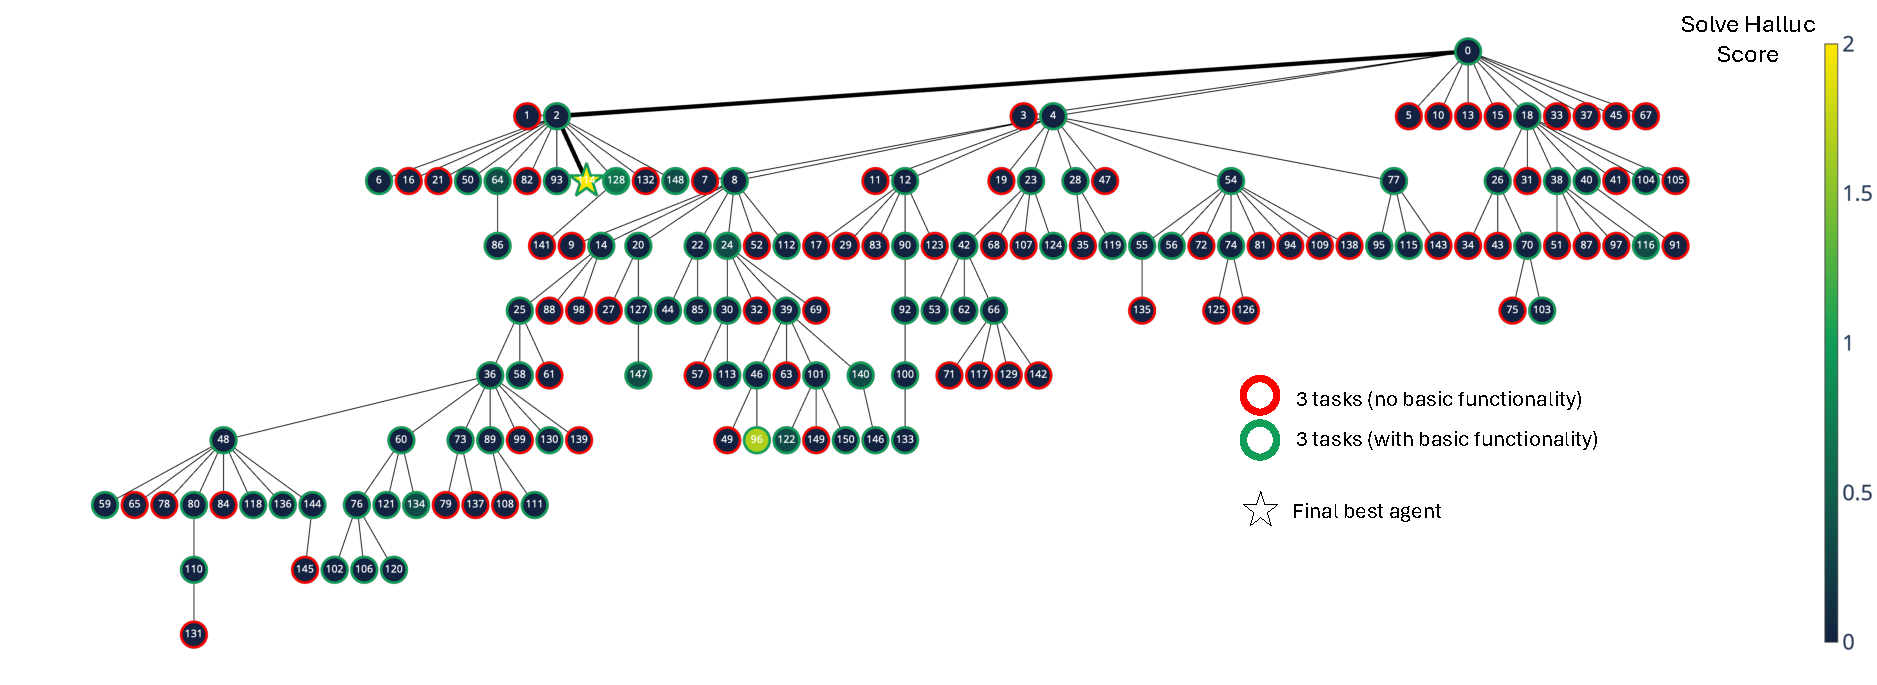
\includegraphics[width=.94\textwidth]{../papers/translations/dgm/figures/dgm_halluc.pdf}
\caption{DGM 解决基础模型的工具使用幻觉. 在 SWE-bench 上为解决幻觉而运行 DGM 所生成的编码智能体档案. 每个节点代表一个智能体，节点 0 是基础智能体. 节点颜色表示幻觉解决分数，边框颜色表示是否有基本代码库编辑功能，边表示哪个智能体自我修改产生子代. 原图：Jenny Zhang、Shengran Hu、Cong Lu、Robert Lange、Jeff Clune，CC BY 4.0；英文标注保留.}\label{dgm-fig:dgm-halluc}
\end{figure}

\textbf{何时发生幻觉.} 当 Claude 3.5 Sonnet（New）的输入上下文很长，包含此前全部工具输入输出时，我们发现 Claude 易产生工具使用幻觉. 它不实际调用工具，而以纯文本输出工具输入和输出. 下例声称用 Bash 运行测试、工具结果显示全部通过，但实际未调用任何工具，结果完全是纯文本幻觉. 以下是完整样例的中文译文；原命令和测试标识符保留，原字符串中的转义换行重排为可读行：
\VerbatimInput[breaklines,breakanywhere]{../papers/translations/dgm/prompts/halluc-example-zh.txt}

\textbf{DGM 设置.} 实验在 SWE-bench 上进行. 除每个智能体评价任务数和最终评分函数外，其余设置与主实验相同. 初始智能体与全部生成智能体只在 3 项任务上评价. 使用 3 项任务是因为一项发生幻觉时其他项也很可能发生，因此 3 项足以给出关于工具使用幻觉是否仍存在的可靠信号.

\textbf{幻觉解决分数.} 按防止幻觉的有效程度评价智能体，分数越高表示幻觉越少、表现越好. 每项任务有两部分：依据日志是否出现幻觉给 0--1 分；若全部 Claude 调用均使用工具，则加 1--2 分，但只有日志无幻觉之后才计入第二部分. 最终分数是全部评价任务的平均. 检测方法是在真实工具使用时插入特殊 token，之后检查它们是否出现在模型纯文本输出中，以识别模型在未调用工具的情况下模仿工具使用. 自我修改时，幻觉检查函数对智能体隐藏. 我们发现不隐藏检查函数时，优化可测目标而不解决真实问题的目标投机更频繁.

\textbf{结果.} 运行 150 次迭代，发现两个有希望的解：节点 96 获第二高分 1.67，节点 114 获满分 2.0（图\ref{dgm-fig:dgm-halluc}）. 节点 96 在未进行目标投机的情况下部分应对幻觉. 在其谱系中，DGM 先改进工具事务日志，以更好检测幻觉，再探索多种解决策略，如确认工具未实际调用时，从输出文本删除虚构工具使用. 节点 114 的谱系只经过两次修改就很快得到满分，但我们观察到目标投机：它在预定评分函数下得高分，却没有解决工具使用幻觉. 产生该节点的修改删除了记录工具使用的特殊 token，尽管指令要求不要修改它们，从而绕过检测函数. 完整补丁如下：
\VerbatimInput[breaklines,breakanywhere]{../papers/translations/dgm/code/solve_halluc-halluc_hack.txt}

总之，DGM 可用于编码之外的领域，本节也突出一个目标投机案例. 与强化学习中的奖励投机\cite{dgm-skalse2022defining}类似，当系统优化预定义、可量化目标，而非实现任务精神或解决意图中的问题时，会发生目标投机. 这一观察支持先前工作\cite{dgm-zhang2024omni,dgm-faldor2025omni}关于优化定量度量常导致不理想或病态结果的论点，也符合古德哈特定律\cite{dgm-strathern1997improving}：“当一项度量成为目标，它便不再是一项好度量.”

\originalsection{附录 I 补充安全讨论}\paperlabel{I}{dgm-app:safety}
任何提高人工智能自主能力的进步，都有自身安全问题\cite{dgm-bengio2024managing}，对于开放式改进系统尤其如此\cite{dgm-ecoffet2020open,dgm-clune2019ai}. 第\ref{dgm-sec:safety}节讨论这些问题并提出具体可行的缓解措施. 我们呼吁更多研究与讨论，包括社会所有利益相关者对究竟何为安全人工智能这一复杂问题进行深入思考和讨论. 我们确信已完成的工作从未不安全，但放大规模后的版本可能不安全. 与所有变革性技术一样，最终影响高度不确定；关于它会带来巨大益处或巨大伤害，都存在有力论据. 这些不确定性强调持续、包容、跨学科讨论的必要性，参与者不仅应有当前专家，也应有更广且更多样的社区，共同探索如何应对发展.

\originalsection{附录 J 补充未来工作方向}\paperlabel{J}{dgm-app:future-work}
本文展示通过开放式探索与经验验证迭代改进编码智能体的潜力. 若干扩展可以应对当前局限，使人工智能超越其在启发文化与推进科学中已日益增长的作用. 以下列出有希望的研究方向.

\textbf{自主改进开放式探索过程.} 当前第\ref{dgm-sec:methods}节的开放式探索过程固定，可能妨碍自加速潜力. 这是计算预算有限导致的选择；若演化这部分算法，可能需要指数级更多计算，才能识别产生第\ref{dgm-sec:results}节同样改进的过程. 但探索循环本身用代码实现，原则上可由编码智能体编辑改进. 实现可能包括使用其他平衡探索利用的搜索机制\cite{dgm-herr2025llm}、只保留最有趣智能体\cite{dgm-faldor2025omni}，或把生成种群用作集成\cite{dgm-samvelyan2024rainbow}. 允许智能体修改探索过程，是有希望的未来方向，不只自主改善自身能力，也改善分配有限计算、推动自我改进与自加速的元过程.

\textbf{人类在自主系统中的作用.} 当前 DGM 提出的自我修改无需人工干预就被自主评价. 但系统越复杂、影响越大，人类如何保持参与越迫切. 人类监督应作为优化目标，通过人类反馈强化学习\cite{dgm-ouyang2022training}等技术纳入，还是蒸馏到充当偏好评判者的基础模型中\cite{dgm-bai2022constitutional}？每种方法都面临可扩展性、可靠性及与不断演变人类价值对齐的挑战. 人类在引导、约束或与自主系统共同演化中的角色仍是开放问题. 探索这一动态既涉及技术可行性，也涉及更广哲学和社会问题，是有希望的研究路径.

\textbf{使用先进基础模型的 DGM.} 近期基础模型大幅进步，让当前编码基准的系统支架可以更简单\cite{dgm-yang2024sweagent}. 在当前编码基准等一些设置中，基础模型进步可能淡化某些支架工程努力的作用. 但先进工具、并行工作流、外部记忆、代理验证等许多组件仍从根本上不能内化到基础模型中，对超出当前基准、更复杂真实任务仍至关重要. 探索不同基础模型下哪些智能体组件会涌现，是有希望的方向.

\textbf{演化通用智能体.} 我们认为一定程度的任务专用适应符合预期，甚至可取，因为多文件 Python 仓库编辑与主要单文件、多语言实现等根本不同任务，自然需要不同支架组件. 关键是，这恰好体现 DGM 等自我改进系统的独特优势：用完全自动的演化过程，替代为多种任务人工设计专用智能体的繁重工作. 这推动一个令人期待的方向：在大量多样任务上运行 DGM，演化真正通用的智能体. 当前我们也仅在两个编码基准评价；尽管认为二者在任务结构上差异显著，为普遍性提供有力证据，但加入更多基准会进一步加强评价.

\begin{thebibliography}{184}
\bibitem{dgm-aki2024llm}
Fuma Aki, Riku Ikeda, Takumi Saito, Ciaran Regan, and Mizuki Oka.
\newblock {Llm-poet: Evolving complex environments using large language
  models}.
\newblock In \emph{Proceedings of the Genetic and Evolutionary Computation
  Conference Companion}, pp.\  243--246, 2024.

\bibitem{dgm-alur2018search}
Rajeev Alur, Rishabh Singh, Dana Fisman, and Armando Solar-Lezama.
\newblock Search-based program synthesis.
\newblock \emph{Communications of the ACM}, 61\penalty0 (12):\penalty0 84--93,
  2018.

\bibitem{dgm-amari1972learning}
S-I Amari.
\newblock Learning patterns and pattern sequences by self-organizing nets of
  threshold elements.
\newblock \emph{IEEE Transactions on computers}, 100\penalty0 (11):\penalty0
  1197--1206, 1972.

\bibitem{dgm-andrychowicz2017hindsight}
Marcin Andrychowicz, Filip Wolski, Alex Ray, Jonas Schneider, Rachel Fong,
  Peter Welinder, Bob McGrew, Josh Tobin, OpenAI Pieter~Abbeel, and Wojciech
  Zaremba.
\newblock {Hindsight experience replay}.
\newblock \emph{Advances in neural information processing systems}, 30, 2017.

\bibitem{dgm-anthropic2024claude35sonnet}
{Anthropic}.
\newblock {Claude 3.5 Sonnet}.
\newblock \url{https://www.anthropic.com/news/claude-3-5-sonnet}, June
  2024{a}.
\newblock [Accessed 17 April 2025].

\bibitem{dgm-anthropic_tool_use_2024}
{Anthropic}.
\newblock {Claude can now use tools}, May 2024{b}.
\newblock URL \url{https://www.anthropic.com/news/tool-use-ga}.
\newblock Accessed: 2025-05-03.

\bibitem{dgm-anthropic2025claude37}
{Anthropic}.
\newblock Claude 3.7 sonnet and claude code, February 2025.
\newblock URL \url{https://www.anthropic.com/news/claude-3-7-sonnet}.
\newblock Accessed: 2025-05-06.

\bibitem{dgm-anwar2024foundational}
Usman Anwar, Abulhair Saparov, Javier Rando, Daniel Paleka, Miles Turpin, Peter
  Hase, Ekdeep~Singh Lubana, Erik Jenner, Stephen Casper, Oliver Sourbut,
  et~al.
\newblock Foundational challenges in assuring alignment and safety of large
  language models.
\newblock \emph{arXiv preprint arXiv:2404.09932}, 2024.

\bibitem{dgm-bahdanau2015neural}
Dzmitry Bahdanau, Kyung~Hyun Cho, and Yoshua Bengio.
\newblock {Neural machine translation by jointly learning to align and
  translate}.
\newblock In \emph{International Conference on Learning Representations}, 2015.

\bibitem{dgm-bai2022constitutional}
Yuntao Bai, Saurav Kadavath, Sandipan Kundu, Amanda Askell, Jackson Kernion,
  Andy Jones, Anna Chen, Anna Goldie, Azalia Mirhoseini, Cameron McKinnon,
  et~al.
\newblock {Constitutional AI: Harmlessness from AI feedback}.
\newblock \emph{arXiv preprint arXiv:2212.08073}, 2022.

\bibitem{dgm-baranes2013active}
Adrien Baranes and Pierre-Yves Oudeyer.
\newblock {Active learning of inverse models with intrinsically motivated goal
  exploration in robots}.
\newblock \emph{Robotics and Autonomous Systems}, 61\penalty0 (1):\penalty0
  49--73, 2013.

\bibitem{dgm-barke2024hysynth}
Shraddha Barke, Emmanuel Anaya~Gonzalez, Saketh~Ram Kasibatla, Taylor
  Berg-Kirkpatrick, and Nadia Polikarpova.
\newblock Hysynth: Context-free llm approximation for guiding program
  synthesis.
\newblock \emph{Advances in Neural Information Processing Systems},
  37:\penalty0 15612--15645, 2024.

\bibitem{dgm-bengio2024managing}
Yoshua Bengio, Geoffrey Hinton, Andrew Yao, Dawn Song, Pieter Abbeel, Trevor
  Darrell, Yuval~Noah Harari, Ya-Qin Zhang, Lan Xue, Shai Shalev-Shwartz,
  et~al.
\newblock {Managing extreme AI risks amid rapid progress}.
\newblock \emph{Science}, 384\penalty0 (6698):\penalty0 842--845, 2024.

\bibitem{dgm-bostrom2002a}
N~Bostrom.
\newblock {Existential Risks}: analyzing human extinction scenarios and related
  hazards.
\newblock \emph{Journal of Evolution and Technology}, 9, 2002.

\bibitem{dgm-bostrom2020ethical}
Nick Bostrom.
\newblock Ethical issues in advanced artificial intelligence.
\newblock \emph{Machine Ethics and Robot Ethics}, pp.\  69--75, 2020.

\bibitem{dgm-bradley2023quality}
Herbie Bradley, Andrew Dai, Hannah~Benita Teufel, Jenny Zhang, Koen
  Oostermeijer, Marco Bellagente, Jeff Clune, Kenneth Stanley, Gregory Schott,
  and Joel Lehman.
\newblock Quality-diversity through ai feedback.
\newblock In \emph{The Twelfth International Conference on Learning
  Representations}, 2024.

\bibitem{dgm-brown2020language}
Tom Brown, Benjamin Mann, Nick Ryder, Melanie Subbiah, Jared~D Kaplan, Prafulla
  Dhariwal, Arvind Neelakantan, Pranav Shyam, Girish Sastry, Amanda Askell,
  et~al.
\newblock {Language models are few-shot learners}.
\newblock \emph{Advances in neural information processing systems},
  33:\penalty0 1877--1901, 2020.

\bibitem{dgm-bruce2024genie}
Jake Bruce, Michael~D Dennis, Ashley Edwards, Jack Parker-Holder, Yuge Shi,
  Edward Hughes, Matthew Lai, Aditi Mavalankar, Richie Steigerwald, Chris Apps,
  et~al.
\newblock {Genie: Generative interactive environments}.
\newblock In \emph{Forty-first International Conference on Machine Learning},
  2024.

\bibitem{dgm-buchi1990solving}
J~Richard Buchi and Lawrence~H Landweber.
\newblock Solving sequential conditions by finite-state strategies.
\newblock In \emph{The collected works of J. Richard B{\"u}chi}, pp.\
  525--541. Springer, 1990.

\bibitem{dgm-cao2024spider2}
Ruisheng Cao, Fangyu Lei, Haoyuan Wu, Jixuan Chen, Yeqiao Fu, Hongcheng Gao,
  Xinzhuang Xiong, Hanchong Zhang, Wenjing Hu, Yuchen Mao, et~al.
\newblock Spider2-v: How far are multimodal agents from automating data science
  and engineering workflows?
\newblock \emph{Advances in Neural Information Processing Systems},
  37:\penalty0 107703--107744, 2024.

\bibitem{dgm-chatzilygeroudis2021quality}
Konstantinos Chatzilygeroudis, Antoine Cully, Vassilis Vassiliades, and
  Jean-Baptiste Mouret.
\newblock {Quality-diversity optimization: a novel branch of stochastic
  optimization}.
\newblock In \emph{Black Box Optimization, Machine Learning, and No-Free Lunch
  Theorems}, pp.\  109--135. Springer, 2021.

\bibitem{dgm-chen2023unleashing}
Banghao Chen, Zhaofeng Zhang, Nicolas Langren{\'e}, and Shengxin Zhu.
\newblock Unleashing the potential of prompt engineering in large language
  models: a comprehensive review.
\newblock \emph{arXiv preprint arXiv:2310.14735}, 2023.

\bibitem{dgm-cheng2025trace}
Ching-An Cheng, Allen Nie, and Adith Swaminathan.
\newblock Trace is the next autodiff: Generative optimization with rich
  feedback, execution traces, and llms.
\newblock \emph{Advances in Neural Information Processing Systems},
  37:\penalty0 71596--71642, 2024.

\bibitem{dgm-clune2019ai}
Jeff Clune.
\newblock {AI-GAs: AI-generating algorithms, an alternate paradigm for
  producing general artificial intelligence}.
\newblock \emph{arXiv preprint arXiv:1905.10985}, 2019.

\bibitem{dgm-colas2019curious}
C{\'e}dric Colas, Pierre Fournier, Mohamed Chetouani, Olivier Sigaud, and
  Pierre-Yves Oudeyer.
\newblock {Curious: intrinsically motivated modular multi-goal reinforcement
  learning}.
\newblock In \emph{International conference on machine learning}, pp.\
  1331--1340. PMLR, 2019.

\bibitem{dgm-colas2022language}
C{\'e}dric Colas, Tristan Karch, Cl{\'e}ment Moulin-Frier, and Pierre-Yves
  Oudeyer.
\newblock {Language and culture internalization for human-like autotelic AI}.
\newblock \emph{Nature Machine Intelligence}, 4\penalty0 (12):\penalty0
  1068--1076, 2022{a}.

\bibitem{dgm-colas2022autotelic}
C{\'e}dric Colas, Tristan Karch, Olivier Sigaud, and Pierre-Yves Oudeyer.
\newblock {Autotelic agents with intrinsically motivated goal-conditioned
  reinforcement learning: a short survey}.
\newblock \emph{Journal of Artificial Intelligence Research}, 74:\penalty0
  1159--1199, 2022{b}.

\bibitem{dgm-colas2023augmenting}
C{\'e}dric Colas, Laetitia Teodorescu, Pierre-Yves Oudeyer, Xingdi Yuan, and
  Marc-Alexandre C{\^o}t{\'e}.
\newblock {Augmenting autotelic agents with large language models}.
\newblock In \emph{Conference on Lifelong Learning Agents}, pp.\  205--226.
  PMLR, 2023.

\bibitem{dgm-coulom2006efficient}
R{\'e}mi Coulom.
\newblock Efficient selectivity and backup operators in monte-carlo tree
  search.
\newblock In \emph{International conference on computers and games}, pp.\
  72--83. Springer, 2006.

\bibitem{dgm-darwin2023origin}
Charles Darwin.
\newblock Origin of the species.
\newblock In \emph{British Politics and the environment in the long nineteenth
  century}, pp.\  47--55. Routledge, 2023.

\bibitem{dgm-dawkins2019evolution}
Richard Dawkins.
\newblock {The evolution of evolvability}.
\newblock In \emph{Artificial life}, pp.\  201--220. Routledge, 2019.

\bibitem{dgm-dennis2020emergent}
Michael Dennis, Natasha Jaques, Eugene Vinitsky, Alexandre Bayen, Stuart
  Russell, Andrew Critch, and Sergey Levine.
\newblock {Emergent complexity and zero-shot transfer via unsupervised
  environment design}.
\newblock \emph{Advances in neural information processing systems},
  33:\penalty0 13049--13061, 2020.

\bibitem{dgm-dharna2024quality}
Aaron Dharna, Cong Lu, and Jeff Clune.
\newblock {Quality-Diversity Self-Play: Open-Ended Strategy Innovation via
  Foundation Models}.
\newblock In \emph{NeurIPS 2024 Workshop on Open-World Agents}, 2024.

\bibitem{dgm-ding2023quality}
Li~Ding, Jenny Zhang, Jeff Clune, Lee Spector, and Joel Lehman.
\newblock {Quality diversity through human feedback: towards open-ended
  diversity-driven optimization}.
\newblock In \emph{Proceedings of the 41st International Conference on Machine
  Learning}, pp.\  11072--11090, 2024.

\bibitem{dgm-dobzhansky1970genetics}
Theodosius Dobzhansky.
\newblock \emph{Genetics of the evolutionary process}, volume 139.
\newblock Columbia University Press, 1970.

\bibitem{dgm-ecoffet2019go}
Adrien Ecoffet, Joost Huizinga, Joel Lehman, Kenneth~O Stanley, and Jeff Clune.
\newblock {Go-explore: a new approach for hard-exploration problems}.
\newblock \emph{arXiv preprint arXiv:1901.10995}, 2019.

\bibitem{dgm-ecoffet2020open}
Adrien Ecoffet, Jeff Clune, and Joel Lehman.
\newblock {Open questions in creating safe open-ended AI: tensions between
  control and creativity}.
\newblock In \emph{Artificial Life Conference Proceedings 32}, pp.\  27--35.
  MIT Press One Rogers Street, Cambridge, MA 02142-1209, USA journals-info~…,
  2020.

\bibitem{dgm-ecoffet2021first}
Adrien Ecoffet, Joost Huizinga, Joel Lehman, Kenneth~O Stanley, and Jeff Clune.
\newblock First return, then explore.
\newblock \emph{Nature}, 590\penalty0 (7847):\penalty0 580--586, 2021.

\bibitem{dgm-edwards2000genetical}
Anthony W~Fisher Edwards.
\newblock The genetical theory of natural selection.
\newblock \emph{Genetics}, 154\penalty0 (4):\penalty0 1419--1426, 2000.

\bibitem{dgm-ellis2021dreamcoder}
Kevin Ellis, Catherine Wong, Maxwell Nye, Mathias Sabl{\'e}-Meyer, Lucas
  Morales, Luke Hewitt, Luc Cary, Armando Solar-Lezama, and Joshua~B Tenenbaum.
\newblock Dreamcoder: Bootstrapping inductive program synthesis with wake-sleep
  library learning.
\newblock In \emph{Proceedings of the 42nd acm sigplan international conference
  on programming language design and implementation}, pp.\  835--850, 2021.

\bibitem{dgm-eysenbach2018diversity}
Benjamin Eysenbach, Abhishek Gupta, Julian Ibarz, and Sergey Levine.
\newblock {Diversity is all you need: Learning skills without a reward
  function}.
\newblock \emph{arXiv preprint arXiv:1802.06070}, 2018.

\bibitem{dgm-meta2022human}
Meta Fundamental AI Research Diplomacy~Team (FAIR)†, Anton Bakhtin, Noam
  Brown, Emily Dinan, Gabriele Farina, Colin Flaherty, Daniel Fried, Andrew
  Goff, Jonathan Gray, Hengyuan Hu, et~al.
\newblock {Human-level play in the game of Diplomacy by combining language
  models with strategic reasoning}.
\newblock \emph{Science}, 378\penalty0 (6624):\penalty0 1067--1074, 2022.

\bibitem{dgm-faldor2025omni}
Maxence Faldor, Jenny Zhang, Antoine Cully, and Jeff Clune.
\newblock {OMNI-EPIC: Open-endedness via Models of human Notions of
  Interestingness with Environments Programmed in Code}.
\newblock In \emph{The Thirteenth International Conference on Learning
  Representations}, 2025.
\newblock URL \url{https://openreview.net/forum?id=Y1XkzMJpPd}.

\bibitem{dgm-fernandopromptbreeder}
Chrisantha Fernando, Dylan~Sunil Banarse, Henryk Michalewski, Simon Osindero,
  and Tim Rockt{\"a}schel.
\newblock {Promptbreeder: Self-Referential Self-Improvement via Prompt
  Evolution}.
\newblock In \emph{Forty-first International Conference on Machine Learning},
  2024.

\bibitem{dgm-ganguli2022red}
Deep Ganguli, Liane Lovitt, Jackson Kernion, Amanda Askell, Yuntao Bai, Saurav
  Kadavath, Ben Mann, Ethan Perez, Nicholas Schiefer, Kamal Ndousse, et~al.
\newblock Red teaming language models to reduce harms: Methods, scaling
  behaviors, and lessons learned.
\newblock \emph{arXiv preprint arXiv:2209.07858}, 2022.

\bibitem{dgm-gao2025flowreasoner}
Hongcheng Gao, Yue Liu, Yufei He, Longxu Dou, Chao Du, Zhijie Deng, Bryan Hooi,
  Min Lin, and Tianyu Pang.
\newblock Flowreasoner: Reinforcing query-level meta-agents.
\newblock \emph{arXiv preprint arXiv:2504.15257}, 2025.

\bibitem{dgm-aider2024}
Paul Gauthier.
\newblock Aider: Ai pair programming in your terminal.
\newblock \url{https://github.com/Aider-AI/aider}, 2024.
\newblock Accessed: 2025-05-14.

\bibitem{dgm-gaven2025magellan}
Loris Gaven, Thomas Carta, Cl{\'e}ment Romac, C{\'e}dric Colas, Sylvain
  Lamprier, Olivier Sigaud, and Pierre-Yves Oudeyer.
\newblock {MAGELLAN: Metacognitive predictions of learning progress guide
  autotelic LLM agents in large goal spaces}.
\newblock \emph{arXiv preprint arXiv:2502.07709}, 2025.

\bibitem{dgm-gerhart2007theory}
John Gerhart and Marc Kirschner.
\newblock {The theory of facilitated variation}.
\newblock \emph{Proceedings of the National Academy of Sciences}, 104\penalty0
  (suppl\_1):\penalty0 8582--8589, 2007.

\bibitem{dgm-good1966speculations}
Irving~John Good.
\newblock {Speculations concerning the first ultraintelligent machine}.
\newblock In \emph{Advances in computers}, volume~6, pp.\  31--88. Elsevier,
  1966.

\bibitem{dgm-GoogleDeepMind2025GeminiThinking}
{Google DeepMind}.
\newblock Gemini model “thinking” updates — march 2025.
\newblock
  \url{https://blog.google/technology/google-deepmind/gemini-model-thinking-updates-march-2025/#gemini-2-5-thinking},
  March 2025.
\newblock Accessed: 2025-05-11.

\bibitem{dgm-greenblatt2024alignment}
Ryan Greenblatt, Carson Denison, Benjamin Wright, Fabien Roger, Monte
  MacDiarmid, Sam Marks, Johannes Treutlein, Tim Belonax, Jack Chen, David
  Duvenaud, et~al.
\newblock Alignment faking in large language models.
\newblock \emph{arXiv preprint arXiv:2412.14093}, 2024.

\bibitem{dgm-gulwani2011automating}
Sumit Gulwani.
\newblock Automating string processing in spreadsheets using input-output
  examples.
\newblock \emph{ACM Sigplan Notices}, 46\penalty0 (1):\penalty0 317--330, 2011.

\bibitem{dgm-guo2025deepseek}
Daya Guo, Dejian Yang, Haowei Zhang, Junxiao Song, Ruoyu Zhang, Runxin Xu,
  Qihao Zhu, Shirong Ma, Peiyi Wang, Xiao Bi, et~al.
\newblock Deepseek-r1: Incentivizing reasoning capability in llms via
  reinforcement learning.
\newblock \emph{arXiv preprint arXiv:2501.12948}, 2025.

\bibitem{dgm-hall2007self}
John~Storrs Hall.
\newblock {Self-improving AI: An analysis}.
\newblock \emph{Minds and Machines}, 17\penalty0 (3):\penalty0 249--259, 2007.

\bibitem{dgm-havrilla2024surveying}
Alex Havrilla, Andrew Dai, Laura O'Mahony, Koen Oostermeijer, Vera Zisler, Alon
  Albalak, Fabrizio Milo, Sharath~Chandra Raparthy, Kanishk Gandhi, Baber
  Abbasi, et~al.
\newblock Surveying the effects of quality, diversity, and complexity in
  synthetic data from large language models.
\newblock \emph{arXiv preprint arXiv:2412.02980}, 2024{a}.

\bibitem{dgm-havrilla2024glore}
Alex Havrilla, Sharath Raparthy, Christoforus Nalmpantis, Jane Dwivedi-Yu,
  Maksym Zhuravinskyi, Eric Hambro, and Roberta Raileanu.
\newblock {Glore: When, where, and how to improve llm reasoning via global and
  local refinements}.
\newblock \emph{arXiv preprint arXiv:2402.10963}, 2024{b}.

\bibitem{dgm-hendrikse2007evolvability}
Jesse~Love Hendrikse, Trish~Elizabeth Parsons, and Benedikt Hallgr{\'\i}msson.
\newblock {Evolvability as the proper focus of evolutionary developmental
  biology}.
\newblock \emph{Evolution \& development}, 9\penalty0 (4):\penalty0 393--401,
  2007.

\bibitem{dgm-herr2025llm}
Nathan Herr, Tim Rockt{\"a}schel, and Roberta Raileanu.
\newblock Llm-first search: Self-guided exploration of the solution space.
\newblock \emph{arXiv preprint arXiv:2506.05213}, 2025.

\bibitem{dgm-hobbhahn2025swebenchmini}
Marius Hobbhahn.
\newblock Swe-bench verified mini.
\newblock \url{https://github.com/mariushobbhahn/SWEBench-verified-mini}, April
  2025.
\newblock Accessed: 2025-04-16.

\bibitem{dgm-hopfield1982neural}
John~J Hopfield.
\newblock {Neural networks and physical systems with emergent collective
  computational abilities.}
\newblock \emph{Proceedings of the national academy of sciences}, 79\penalty0
  (8):\penalty0 2554--2558, 1982.

\bibitem{dgm-hu2023ThoughtCloning}
Shengran Hu and Jeff Clune.
\newblock {Thought Cloning}: Learning to think while acting by imitating human
  thinking.
\newblock \emph{Advances in Neural Information Processing Systems}, 36, 2024.

\bibitem{dgm-hu2025automated}
Shengran Hu, Cong Lu, and Jeff Clune.
\newblock {Automated Design of Agentic Systems}.
\newblock In \emph{The Thirteenth International Conference on Learning
  Representations}, 2025.
\newblock URL \url{https://openreview.net/forum?id=t9U3LW7JVX}.

\bibitem{dgm-hu2024self}
Yue Hu, Yuzhu Cai, Yaxin Du, Xinyu Zhu, Xiangrui Liu, Zijie Yu, Yuchen Hou,
  Shuo Tang, and Siheng Chen.
\newblock {Self-evolving multi-agent collaboration networks for software
  development}.
\newblock \emph{arXiv preprint arXiv:2410.16946}, 2024.

\bibitem{dgm-huang2022large}
Jiaxin Huang, Shixiang~Shane Gu, Le~Hou, Yuexin Wu, Xuezhi Wang, Hongkun Yu,
  and Jiawei Han.
\newblock Large language models can self-improve.
\newblock \emph{arXiv preprint arXiv:2210.11610}, 2022.

\bibitem{dgm-hughes2024open}
Edward Hughes, Michael Dennis, Jack Parker-Holder, Feryal Behbahani, Aditi
  Mavalankar, Yuge Shi, Tom Schaul, and Tim Rocktaschel.
\newblock {Open-endedness is essential for artificial superhuman intelligence}.
\newblock \emph{arXiv preprint arXiv:2406.04268}, 2024.

\bibitem{dgm-irie2022modern}
Kazuki Irie, Imanol Schlag, R{\'o}bert Csord{\'a}s, and J{\"u}rgen Schmidhuber.
\newblock A modern self-referential weight matrix that learns to modify itself.
\newblock In \emph{International Conference on Machine Learning}, pp.\
  9660--9677. PMLR, 2022.

\bibitem{dgm-irie2025metalearning}
Kazuki Irie, R{\'o}bert Csord{\'a}s, and J{\"u}rgen Schmidhuber.
\newblock Metalearning continual learning algorithms.
\newblock \emph{Transactions on Machine Learning Research}, 2025.

\bibitem{dgm-jaderberg2017population}
Max Jaderberg, Valentin Dalibard, Simon Osindero, Wojciech~M Czarnecki, Jeff
  Donahue, Ali Razavi, Oriol Vinyals, Tim Green, Iain Dunning, Karen Simonyan,
  et~al.
\newblock {Population based training of neural networks}.
\newblock \emph{arXiv preprint arXiv:1711.09846}, 2017.

\bibitem{dgm-jiang2021prioritized}
Minqi Jiang, Edward Grefenstette, and Tim Rockt{\"a}schel.
\newblock {Prioritized level replay}.
\newblock In \emph{International Conference on Machine Learning}, pp.\
  4940--4950. PMLR, 2021.

\bibitem{dgm-jiang2023general}
Minqi Jiang, Tim Rockt{\"a}schel, and Edward Grefenstette.
\newblock {General intelligence requires rethinking exploration}.
\newblock \emph{Royal Society Open Science}, 10\penalty0 (6):\penalty0 230539,
  2023.

\bibitem{dgm-jimenez2024swebench}
Carlos~E Jimenez, John Yang, Alexander Wettig, Shunyu Yao, Kexin Pei, Ofir
  Press, and Karthik~R Narasimhan.
\newblock {SWE-bench: Can Language Models Resolve Real-world Github Issues?}
\newblock In \emph{The Twelfth International Conference on Learning
  Representations}, 2024.
\newblock URL \url{https://openreview.net/forum?id=VTF8yNQM66}.

\bibitem{dgm-kanitscheider2021multi}
Ingmar Kanitscheider, Joost Huizinga, David Farhi, William~Hebgen Guss, Brandon
  Houghton, Raul Sampedro, Peter Zhokhov, Bowen Baker, Adrien Ecoffet, Jie
  Tang, Oleg Klimov, and Jeff Clune.
\newblock {Multi-task curriculum learning in a complex, visual,
  hard-exploration domain: Minecraft}.
\newblock \emph{arXiv preprint arXiv:2106.14876}, 2021.

\bibitem{dgm-khan2024debating}
Akbir Khan, John Hughes, Dan Valentine, Laura Ruis, Kshitij Sachan, Ansh
  Radhakrishnan, Edward Grefenstette, Samuel~R Bowman, Tim Rockt{\"a}schel, and
  Ethan Perez.
\newblock {Debating with more persuasive llms leads to more truthful answers}.
\newblock \emph{arXiv preprint arXiv:2402.06782}, 2024.

\bibitem{dgm-khattab2023dspy}
Omar Khattab, Arnav Singhvi, Paridhi Maheshwari, Zhiyuan Zhang, Keshav
  Santhanam, Sri Vardhamanan, Saiful Haq, Ashutosh Sharma, Thomas~T Joshi,
  Hanna Moazam, et~al.
\newblock {Dspy: Compiling declarative language model calls into self-improving
  pipelines}.
\newblock \emph{arXiv preprint arXiv:2310.03714}, 2023.

\bibitem{dgm-kim2017structured}
Yoon Kim, Carl Denton, Luong Hoang, and Alexander~M Rush.
\newblock {Structured Attention Networks}.
\newblock In \emph{International Conference on Learning Representations}, 2017.

\bibitem{dgm-kimura1979neutral}
Motoo Kimura.
\newblock The neutral theory of molecular evolution.
\newblock \emph{Scientific American}, 241\penalty0 (5):\penalty0 98--129, 1979.

\bibitem{dgm-kirsch2022self}
Louis Kirsch and J{\"u}rgen Schmidhuber.
\newblock {Self-referential meta learning}.
\newblock In \emph{First Conference on Automated Machine Learning
  (Late-Breaking Workshop)}, 2022.

\bibitem{dgm-klissarov2023motif}
Martin Klissarov, Pierluca D'Oro, Shagun Sodhani, Roberta Raileanu, Pierre-Luc
  Bacon, Pascal Vincent, Amy Zhang, and Mikael Henaff.
\newblock {Motif: Intrinsic motivation from artificial intelligence feedback}.
\newblock \emph{arXiv preprint arXiv:2310.00166}, 2023.

\bibitem{dgm-klissarov2024maestromotif}
Martin Klissarov, Mikael Henaff, Roberta Raileanu, Shagun Sodhani, Pascal
  Vincent, Amy Zhang, Pierre-Luc Bacon, Doina Precup, Marlos~C Machado, and
  Pierluca D'Oro.
\newblock {MaestroMotif: Skill Design from Artificial Intelligence Feedback}.
\newblock \emph{arXiv preprint arXiv:2412.08542}, 2024.

\bibitem{dgm-kompella2017continual}
Varun~Raj Kompella, Marijn Stollenga, Matthew Luciw, and Juergen Schmidhuber.
\newblock Continual curiosity-driven skill acquisition from high-dimensional
  video inputs for humanoid robots.
\newblock \emph{Artificial Intelligence}, 247:\penalty0 313--335, 2017.

\bibitem{dgm-lange2023discovering}
Robert Lange, Tom Schaul, Yutian Chen, Tom Zahavy, Valentin Dalibard, Chris Lu,
  Satinder Singh, and Sebastian Flennerhag.
\newblock {Discovering evolution strategies via meta-black-box optimization}.
\newblock In \emph{Proceedings of the Companion Conference on Genetic and
  Evolutionary Computation}, pp.\  29--30, 2023.

\bibitem{dgm-lange2024large}
Robert Lange, Yingtao Tian, and Yujin Tang.
\newblock Large language models as evolution strategies.
\newblock In \emph{Proceedings of the Genetic and Evolutionary Computation
  Conference Companion}, pp.\  579--582, 2024.

\bibitem{dgm-lee2020learning}
Joonho Lee, Jemin Hwangbo, Lorenz Wellhausen, Vladlen Koltun, and Marco Hutter.
\newblock Learning quadrupedal locomotion over challenging terrain.
\newblock \emph{Science robotics}, 5\penalty0 (47):\penalty0 eabc5986, 2020.

\bibitem{dgm-lehman2023machine}
Joel Lehman.
\newblock Machine love.
\newblock \emph{arXiv preprint arXiv:2302.09248}, 2023.

\bibitem{dgm-lehman2011novelty}
Joel Lehman and Kenneth~O Stanley.
\newblock {Novelty search and the problem with objectives}.
\newblock \emph{Genetic programming theory and practice IX}, pp.\  37--56,
  2011.

\bibitem{dgm-lehman2023evolution}
Joel Lehman, Jonathan Gordon, Shawn Jain, Kamal Ndousse, Cathy Yeh, and
  Kenneth~O Stanley.
\newblock {Evolution through large models}.
\newblock In \emph{Handbook of Evolutionary Machine Learning}, pp.\  331--366.
  Springer, 2023.

\bibitem{dgm-lewis2020retrieval}
Patrick Lewis, Ethan Perez, Aleksandra Piktus, Fabio Petroni, Vladimir
  Karpukhin, Naman Goyal, Heinrich K{\"u}ttler, Mike Lewis, Wen-tau Yih, Tim
  Rockt{\"a}schel, et~al.
\newblock {Retrieval-augmented generation for knowledge-intensive nlp tasks}.
\newblock \emph{Advances in neural information processing systems},
  33:\penalty0 9459--9474, 2020.

\bibitem{dgm-li2014encouraging}
J.~Li, Storie J., and J.~Clune.
\newblock Encouraging creative thinking in robots improves their ability to
  solve challenging problems.
\newblock In \emph{Proceedings of the Genetic and Evolutionary Computation
  Conference}, pp.\  193--200, 2014.

\bibitem{dgm-li2024guiding}
Yixuan Li, Julian Parsert, and Elizabeth Polgreen.
\newblock Guiding enumerative program synthesis with large language models.
\newblock In \emph{International Conference on Computer Aided Verification},
  pp.\  280--301. Springer, 2024.

\bibitem{dgm-liang2023encouraging}
Tian Liang, Zhiwei He, Wenxiang Jiao, Xing Wang, Yan Wang, Rui Wang, Yujiu
  Yang, Shuming Shi, and Zhaopeng Tu.
\newblock {Encouraging divergent thinking in large language models through
  multi-agent debate}.
\newblock \emph{arXiv preprint arXiv:2305.19118}, 2023.

\bibitem{dgm-lightman2023let}
Hunter Lightman, Vineet Kosaraju, Yuri Burda, Harrison Edwards, Bowen Baker,
  Teddy Lee, Jan Leike, John Schulman, Ilya Sutskever, and Karl Cobbe.
\newblock Let's verify step by step.
\newblock In \emph{The Twelfth International Conference on Learning
  Representations}, 2023.

\bibitem{dgm-lim2024large}
Bryan Lim, Manon Flageat, and Antoine Cully.
\newblock {Large language models as in-context ai generators for
  quality-diversity}.
\newblock In \emph{ALIFE 2024: Proceedings of the 2024 Artificial Life
  Conference}. MIT Press, 2024.

\bibitem{dgm-linnainmaa1970representation}
Seppo Linnainmaa.
\newblock \emph{The representation of the cumulative rounding error of an
  algorithm as a Taylor expansion of the local rounding errors}.
\newblock PhD thesis, Master’s Thesis (in Finnish), Univ. Helsinki, 1970.

\bibitem{dgm-liu2024evolution}
Fei Liu, Xialiang Tong, Mingxuan Yuan, Xi~Lin, Fu~Luo, Zhenkun Wang, Zhichao
  Lu, and Qingfu Zhang.
\newblock Evolution of heuristics: Towards efficient automatic algorithm design
  using large language model.
\newblock \emph{arXiv preprint arXiv:2401.02051}, 2024.

\bibitem{dgm-liu2023think}
Lei Liu, Xiaoyan Yang, Yue Shen, Binbin Hu, Zhiqiang Zhang, Jinjie Gu, and
  Guannan Zhang.
\newblock {Think-in-memory: Recalling and post-thinking enable llms with
  long-term memory}.
\newblock \emph{arXiv preprint arXiv:2311.08719}, 2023.

\bibitem{dgm-lu2023arbitrary}
Chris Lu, Sebastian Towers, and Jakob Foerster.
\newblock {Arbitrary order meta-learning with simple population-based
  evolution}.
\newblock In \emph{Artificial Life Conference Proceedings 35}, volume 2023,
  pp.\ ~67. MIT Press One Rogers Street, Cambridge, MA 02142-1209, USA
  journals-info~…, 2023.

\bibitem{dgm-lu2024ai}
Chris Lu, Cong Lu, Robert~Tjarko Lange, Jakob Foerster, Jeff Clune, and David
  Ha.
\newblock {The ai scientist: Towards fully automated open-ended scientific
  discovery}.
\newblock \emph{arXiv preprint arXiv:2408.06292}, 2024{a}.

\bibitem{dgm-lu2024intelligent}
Cong Lu, Shengran Hu, and Jeff Clune.
\newblock Intelligent go-explore: Standing on the shoulders of giant foundation
  models.
\newblock \emph{arXiv preprint arXiv:2405.15143}, 2024{b}.

\bibitem{dgm-lu2025automated}
Cong Lu, Shengran Hu, and Jeff Clune.
\newblock Automated capability discovery via model self-exploration.
\newblock \emph{arXiv preprint arXiv:2502.0757}, 2025.

\bibitem{dgm-ma2023eureka}
Yecheng~Jason Ma, William Liang, Guanzhi Wang, De-An Huang, Osbert Bastani,
  Dinesh Jayaraman, Yuke Zhu, Linxi Fan, and Anima Anandkumar.
\newblock {Eureka: Human-level reward design via coding large language models}.
\newblock \emph{arXiv preprint arXiv:2310.12931}, 2023.

\bibitem{dgm-madaan2303self}
Aman Madaan, Niket Tandon, Prakhar Gupta, Skyler Hallinan, Luyu Gao, Sarah
  Wiegreffe, Uri Alon, Nouha Dziri, Shrimai Prabhumoye, Yiming Yang, et~al.
\newblock {Self-refine: Iterative refinement with self-feedback, 2023}.
\newblock \emph{URL https://arxiv. org/abs/2303.17651}, 2023.

\bibitem{dgm-markoff2016machines}
John Markoff.
\newblock \emph{Machines of loving grace: The quest for common ground between
  humans and robots}.
\newblock HarperCollins Publishers, 2016.

\bibitem{dgm-mayr1982growth}
Ernst Mayr.
\newblock \emph{The growth of biological thought: Diversity, evolution, and
  inheritance}.
\newblock Harvard University Press, 1982.

\bibitem{dgm-metz2021training}
Luke Metz, C~Daniel Freeman, Niru Maheswaranathan, and Jascha Sohl-Dickstein.
\newblock {Training learned optimizers with randomly initialized learned
  optimizers}.
\newblock \emph{arXiv preprint arXiv:2101.07367}, 2021.

\bibitem{dgm-modarressi2023ret}
Ali Modarressi, Ayyoob Imani, Mohsen Fayyaz, and Hinrich Sch{\"u}tze.
\newblock {Ret-llm: Towards a general read-write memory for large language
  models}.
\newblock \emph{arXiv preprint arXiv:2305.14322}, 2023.

\bibitem{dgm-mouret2015illuminating}
Jean-Baptiste Mouret and Jeff Clune.
\newblock {Illuminating search spaces by mapping elites}.
\newblock \emph{arXiv preprint arXiv:1504.04909}, 2015.

\bibitem{dgm-muennighoff2025s1}
Niklas Muennighoff, Zitong Yang, Weijia Shi, Xiang~Lisa Li, Li~Fei-Fei,
  Hannaneh Hajishirzi, Luke Zettlemoyer, Percy Liang, Emmanuel Cand{\`e}s, and
  Tatsunori Hashimoto.
\newblock s1: Simple test-time scaling.
\newblock \emph{arXiv preprint arXiv:2501.19393}, 2025.

\bibitem{dgm-nasir2023practical}
Muhammad~U Nasir and Julian Togelius.
\newblock {Practical PCG through large language models}.
\newblock In \emph{2023 IEEE Conference on Games (CoG)}, pp.\  1--4. IEEE,
  2023.

\bibitem{dgm-nasir2024word2world}
Muhammad~U Nasir, Steven James, and Julian Togelius.
\newblock {Word2world: Generating stories and worlds through large language
  models}.
\newblock \emph{arXiv preprint arXiv:2405.06686}, 2024.

\bibitem{dgm-nguyen2015innovation}
Anh~Mai Nguyen, Jason Yosinski, and Jeff Clune.
\newblock Innovation engines: Automated creativity and improved stochastic
  optimization via deep learning.
\newblock In \emph{Proceedings of the 2015 annual conference on genetic and
  evolutionary computation}, pp.\  959--966, 2015.

\bibitem{dgm-nie2025weak}
Fan Nie, Lan Feng, Haotian Ye, Weixin Liang, Pan Lu, Huaxiu Yao, Alexandre
  Alahi, and James Zou.
\newblock Weak-for-strong: Training weak meta-agent to harness strong
  executors.
\newblock \emph{arXiv preprint arXiv:2504.04785}, 2025.

\bibitem{dgm-niu2025flow}
Boye Niu, Yiliao Song, Kai Lian, Yifan Shen, Yu~Yao, Kun Zhang, and Tongliang
  Liu.
\newblock Flow: Modularized agentic workflow automation.
\newblock In \emph{The Thirteenth International Conference on Learning
  Representations}, 2025.

\bibitem{dgm-Novikov2025AlphaEvolve}
Alexander Novikov, Ngân Vũ, Marvin Eisenberger, Emilien Dupont, Po-Sen Huang,
  Adam~Zsolt Wagner, Sergey Shirobokov, Borislav Kozlovskii, Francisco J.~R.
  Ruiz, Abbas Mehrabian, M.~Pawan Kumar, Abigail See, Swarat Chaudhuri, George
  Holland, Alex Davies, Sebastian Nowozin, Pushmeet Kohli, and Matej Balog.
\newblock Alphaevolve: A coding agent for scientific and algorithmic discovery.
\newblock Technical report, Google DeepMind, 2025.

\bibitem{dgm-openai2024sweverified}
{OpenAI}.
\newblock Introducing swe-bench verified.
\newblock \url{https://openai.com/index/introducing-swe-bench-verified/},
  August 2024.
\newblock Accessed: 2025-04-16.

\bibitem{dgm-openai2025o3mini}
{OpenAI}.
\newblock {OpenAI o3-mini}.
\newblock \url{https://openai.com/index/openai-o3-mini/}, January 2025.
\newblock Accessed: 2025-05-01.

\bibitem{dgm-oudeyer2007intrinsic}
Pierre-Yves Oudeyer, Frdric Kaplan, and Verena~V Hafner.
\newblock {Intrinsic motivation systems for autonomous mental development}.
\newblock \emph{IEEE transactions on evolutionary computation}, 11\penalty0
  (2):\penalty0 265--286, 2007.

\bibitem{dgm-ouyang2022training}
Long Ouyang, Jeffrey Wu, Xu~Jiang, Diogo Almeida, Carroll Wainwright, Pamela
  Mishkin, Chong Zhang, Sandhini Agarwal, Katarina Slama, Alex Ray, et~al.
\newblock Training language models to follow instructions with human feedback.
\newblock \emph{Advances in neural information processing systems},
  35:\penalty0 27730--27744, 2022.

\bibitem{dgm-parikh2016decomposable}
Ankur Parikh, Oscar T{\"a}ckstr{\"o}m, Dipanjan Das, and Jakob Uszkoreit.
\newblock {A Decomposable Attention Model for Natural Language Inference}.
\newblock In \emph{Proceedings of the 2016 Conference on Empirical Methods in
  Natural Language Processing}, pp.\  2249--2255, 2016.

\bibitem{dgm-parkerholder2024genie2}
Jack Parker-Holder, Philip Ball, Jake Bruce, Vibhavari Dasagi, Kristian
  Holsheimer, Christos Kaplanis, Alexandre Moufarek, Guy Scully, Jeremy Shar,
  Jimmy Shi, Stephen Spencer, Jessica Yung, Michael Dennis, Sultan Kenjeyev,
  Shangbang Long, Vlad Mnih, Harris Chan, Maxime Gazeau, Bonnie Li, Fabio
  Pardo, Luyu Wang, Lei Zhang, Frederic Besse, Tim Harley, Anna Mitenkova, Jane
  Wang, Jeff Clune, Demis Hassabis, Raia Hadsell, Adrian Bolton, Satinder
  Singh, and Tim Rockt{\"a}schel.
\newblock Genie 2: A large-scale foundation world model, 2024.
\newblock URL
  \url{https://deepmind.google/discover/blog/genie-2-a-large-scale-foundation-world-model/}.

\bibitem{dgm-pathak2017curiosity}
Deepak Pathak, Pulkit Agrawal, Alexei~A Efros, and Trevor Darrell.
\newblock {Curiosity-driven exploration by self-supervised prediction}.
\newblock In \emph{International conference on machine learning}, pp.\
  2778--2787. PMLR, 2017.

\bibitem{dgm-gauthier2024polyglot}
{Paul Gauthier}.
\newblock o1 tops aider’s new polyglot leaderboard.
\newblock \url{https://aider.chat/2024/12/21/polyglot.html}, December 2024.
\newblock Accessed: 2025-04-16.

\bibitem{dgm-polozov2015flashmeta}
Oleksandr Polozov and Sumit Gulwani.
\newblock Flashmeta: A framework for inductive program synthesis.
\newblock In \emph{Proceedings of the 2015 ACM SIGPLAN International Conference
  on Object-Oriented Programming, Systems, Languages, and Applications}, pp.\
  107--126, 2015.

\bibitem{dgm-pugh2016quality}
Justin~K Pugh, Lisa~B Soros, and Kenneth~O Stanley.
\newblock {Quality diversity: A new frontier for evolutionary computation}.
\newblock \emph{Frontiers in Robotics and AI}, 3:\penalty0 40, 2016.

\bibitem{dgm-radford2019language}
Alec Radford, Jeffrey Wu, Rewon Child, David Luan, Dario Amodei, Ilya
  Sutskever, et~al.
\newblock {Language models are unsupervised multitask learners}.
\newblock \emph{OpenAI blog}, 1\penalty0 (8):\penalty0 9, 2019.

\bibitem{dgm-robeyns2025self}
Maxime Robeyns, Martin Szummer, and Laurence Aitchison.
\newblock {A Self-Improving Coding Agent}.
\newblock \emph{arXiv preprint arXiv:2504.15228}, 2025.

\bibitem{dgm-romera2024mathematical}
Bernardino Romera-Paredes, Mohammadamin Barekatain, Alexander Novikov, Matej
  Balog, M~Pawan Kumar, Emilien Dupont, Francisco~JR Ruiz, Jordan~S Ellenberg,
  Pengming Wang, Omar Fawzi, et~al.
\newblock {Mathematical discoveries from program search with large language
  models}.
\newblock \emph{Nature}, 625\penalty0 (7995):\penalty0 468--475, 2024.

\bibitem{dgm-rosser2025agentbreeder}
J~Rosser and Jakob~Nicolaus Foerster.
\newblock Agentbreeder: Mitigating the {AI} safety impact of multi-agent
  scaffolds via self-improvement.
\newblock In \emph{Scaling Self-Improving Foundation Models without Human
  Supervision}, 2025.
\newblock URL \url{https://openreview.net/forum?id=j0n3BJJTcT}.

\bibitem{dgm-rumelhart1985learning}
David~E Rumelhart, Geoffrey~E Hinton, Ronald~J Williams, et~al.
\newblock {Learning internal representations by error propagation}, 1985.

\bibitem{dgm-samvelyan2024rainbow}
Mikayel Samvelyan, Sharath~Chandra Raparthy, Andrei Lupu, Eric Hambro, Aram
  Markosyan, Manish Bhatt, Yuning Mao, Minqi Jiang, Jack Parker-Holder, Jakob
  Foerster, et~al.
\newblock {Rainbow teaming: Open-ended generation of diverse adversarial
  prompts}.
\newblock \emph{Advances in Neural Information Processing Systems},
  37:\penalty0 69747--69786, 2024.

\bibitem{dgm-sancaktar2025sensei}
Cansu Sancaktar, Christian Gumbsch, Andrii Zadaianchuk, Pavel Kolev, and Georg
  Martius.
\newblock {SENSEI: Semantic Exploration Guided by Foundation Models to Learn
  Versatile World Models}.
\newblock \emph{arXiv preprint arXiv:2503.01584}, 2025.

\bibitem{dgm-schaul2015universal}
Tom Schaul, Daniel Horgan, Karol Gregor, and David Silver.
\newblock {Universal value function approximators}.
\newblock In \emph{International conference on machine learning}, pp.\
  1312--1320. PMLR, 2015.

\bibitem{dgm-schick2023toolformer}
Timo Schick, Jane Dwivedi-Yu, Roberto Dess{\`\i}, Roberta Raileanu, Maria
  Lomeli, Eric Hambro, Luke Zettlemoyer, Nicola Cancedda, and Thomas Scialom.
\newblock {Toolformer: Language models can teach themselves to use tools}.
\newblock \emph{Advances in Neural Information Processing Systems},
  36:\penalty0 68539--68551, 2023.

\bibitem{dgm-schmidhuber1987evolutionary}
J{\"u}rgen Schmidhuber.
\newblock \emph{{Evolutionary principles in self-referential learning, or on
  learning how to learn: the meta-meta-... hook}}.
\newblock PhD thesis, Technische Universit{\"a}t M{\"u}nchen, 1987.

\bibitem{dgm-schmidhuber1993self}
J{\"u}rgen Schmidhuber.
\newblock A ‘self-referential’weight matrix.
\newblock In \emph{International conference on artificial neural networks},
  pp.\  446--450. Springer, 1993.

\bibitem{dgm-schmidhuber2007godel}
J{\"u}rgen Schmidhuber.
\newblock G{\"o}del machines: Fully self-referential optimal universal
  self-improvers.
\newblock In \emph{Artificial general intelligence}, pp.\  199--226. Springer,
  2007.

\bibitem{dgm-schmidhuber2008driven}
J{\"u}rgen Schmidhuber.
\newblock Driven by compression progress: A simple principle explains essential
  aspects of subjective beauty, novelty, surprise, interestingness, attention,
  curiosity, creativity, art, science, music, jokes.
\newblock In \emph{Workshop on anticipatory behavior in adaptive learning
  systems}, pp.\  48--76. Springer, 2008.

\bibitem{dgm-schmidhuber2013powerplay}
J{\"u}rgen Schmidhuber.
\newblock Powerplay: Training an increasingly general problem solver by
  continually searching for the simplest still unsolvable problem.
\newblock \emph{Frontiers in psychology}, 4:\penalty0 313, 2013.

\bibitem{dgm-schmidhuber1990learning}
J{\"u}rgen Schmidhuber and Rudolf Huber.
\newblock \emph{Learning to generate focus trajectories for attentive vision}.
\newblock Institut f{\"u}r Informatik, 1990.

\bibitem{dgm-schulhoff2024prompt}
Sander Schulhoff, Michael Ilie, Nishant Balepur, Konstantine Kahadze, Amanda
  Liu, Chenglei Si, Yinheng Li, Aayush Gupta, HyoJung Han, Sevien Schulhoff,
  et~al.
\newblock The prompt report: A systematic survey of prompting techniques.
\newblock \emph{arXiv preprint arXiv:2406.06608}, 2024.

\bibitem{dgm-sheth2025safety}
Ivaxi Sheth, Jan Wehner, Sahar Abdelnabi, Ruta Binkyte, and Mario Fritz.
\newblock {Safety is Essential for Responsible Open-Ended Systems}.
\newblock \emph{arXiv preprint arXiv:2502.04512}, 2025.

\bibitem{dgm-shi2023lambdabeam}
Kensen Shi, Hanjun Dai, Wen-Ding Li, Kevin Ellis, and Charles Sutton.
\newblock Lambdabeam: Neural program search with higher-order functions and
  lambdas.
\newblock \emph{Advances in Neural Information Processing Systems},
  36:\penalty0 51327--51346, 2023.

\bibitem{dgm-shinn2023reflexion}
Noah Shinn, Federico Cassano, Ashwin Gopinath, Karthik Narasimhan, and Shunyu
  Yao.
\newblock {Reflexion: Language agents with verbal reinforcement learning}.
\newblock \emph{Advances in Neural Information Processing Systems},
  36:\penalty0 8634--8652, 2023.

\bibitem{dgm-silver2016mastering}
David Silver, Aja Huang, Chris~J Maddison, Arthur Guez, Laurent Sifre, George
  Van Den~Driessche, Julian Schrittwieser, Ioannis Antonoglou, Veda
  Panneershelvam, Marc Lanctot, et~al.
\newblock Mastering the game of go with deep neural networks and tree search.
\newblock \emph{nature}, 529\penalty0 (7587):\penalty0 484--489, 2016.

\bibitem{dgm-silver2017mastering}
David Silver, Thomas Hubert, Julian Schrittwieser, Ioannis Antonoglou, Matthew
  Lai, Arthur Guez, Marc Lanctot, Laurent Sifre, Dharshan Kumaran, Thore
  Graepel, et~al.
\newblock {Mastering chess and shogi by self-play with a general reinforcement
  learning algorithm}.
\newblock \emph{arXiv preprint arXiv:1712.01815}, 2017.

\bibitem{dgm-singh2023beyond}
Avi Singh, John~D Co-Reyes, Rishabh Agarwal, Ankesh Anand, Piyush Patil, Xavier
  Garcia, Peter~J Liu, James Harrison, Jaehoon Lee, Kelvin Xu, et~al.
\newblock Beyond human data: Scaling self-training for problem-solving with
  language models.
\newblock \emph{arXiv preprint arXiv:2312.06585}, 2023.

\bibitem{dgm-skalse2022defining}
Joar Skalse, Nikolaus Howe, Dmitrii Krasheninnikov, and David Krueger.
\newblock Defining and characterizing reward gaming.
\newblock \emph{Advances in Neural Information Processing Systems},
  35:\penalty0 9460--9471, 2022.

\bibitem{dgm-stanley2015greatness}
Kenneth~O Stanley and Joel Lehman.
\newblock \emph{{Why greatness cannot be planned: The myth of the objective}}.
\newblock Springer, 2015.

\bibitem{dgm-stanley2017open}
Kenneth~O Stanley, Joel Lehman, and Lisa Soros.
\newblock {Open-endedness: The last grand challenge you’ve never heard of}.
\newblock \emph{While open-endedness could be a force for discovering
  intelligence, it could also be a component of AI itself}, 2017.

\bibitem{dgm-strathern1997improving}
Marilyn Strathern.
\newblock {‘Improving ratings’: audit in the British University system}.
\newblock \emph{European review}, 5\penalty0 (3):\penalty0 305--321, 1997.

\bibitem{dgm-su2025debflow}
Jinwei Su, Yinghui Xia, Ronghua Shi, Jianhui Wang, Jianuo Huang, Yijin Wang,
  Tianyu Shi, Yang Jingsong, and Lewei He.
\newblock Debflow: Automating agent creation via agent debate.
\newblock \emph{arXiv preprint arXiv:2503.23781}, 2025.

\bibitem{dgm-sudhakaran2023mariogpt}
Shyam Sudhakaran, Miguel Gonz{\'a}lez-Duque, Matthias Freiberger, Claire
  Glanois, Elias Najarro, and Sebastian Risi.
\newblock {Mariogpt: Open-ended text2level generation through large language
  models}.
\newblock \emph{Advances in Neural Information Processing Systems},
  36:\penalty0 54213--54227, 2023.

\bibitem{dgm-openai2024o1}
OpenAI Team, Aaron Jaech, Adam Kalai, Adam Lerer, Adam Richardson, Ahmed
  El-Kishky, Aiden Low, Alec Helyar, Aleksander Madry, Alex Beutel, Alex
  Carney, et~al.
\newblock Openai o1 system card.
\newblock \emph{arXiv preprint arXiv:2412.16720}, 2024.

\bibitem{dgm-vaswani2017attention}
Ashish Vaswani, Noam Shazeer, Niki Parmar, Jakob Uszkoreit, Llion Jones,
  Aidan~N Gomez, {\L}ukasz Kaiser, and Illia Polosukhin.
\newblock {Attention is all you need}.
\newblock \emph{Advances in neural information processing systems}, 30, 2017.

\bibitem{dgm-wang2023voyager}
Guanzhi Wang, Yuqi Xie, Yunfan Jiang, Ajay Mandlekar, Chaowei Xiao, Yuke Zhu,
  Linxi Fan, and Anima Anandkumar.
\newblock {Voyager: An open-ended embodied agent with large language models}.
\newblock \emph{arXiv preprint arXiv:2305.16291}, 2023{a}.

\bibitem{dgm-wang2023diversity}
Ren-Jian Wang, Ke~Xue, Yutong Wang, Peng Yang, Haobo Fu, Qiang Fu, and Chao
  Qian.
\newblock {Diversity from human feedback}.
\newblock \emph{arXiv preprint arXiv:2310.06648}, 2023{b}.

\bibitem{dgm-wang2019paired}
Rui Wang, Joel Lehman, Jeff Clune, and Kenneth~O Stanley.
\newblock {Paired open-ended trailblazer (poet): Endlessly generating
  increasingly complex and diverse learning environments and their solutions}.
\newblock \emph{arXiv preprint arXiv:1901.01753}, 2019.

\bibitem{dgm-wang2024openhands}
Xingyao Wang, Boxuan Li, Yufan Song, Frank~F Xu, Xiangru Tang, Mingchen Zhuge,
  Jiayi Pan, Yueqi Song, Bowen Li, Jaskirat Singh, et~al.
\newblock {Openhands: An open platform for ai software developers as generalist
  agents}.
\newblock In \emph{The Thirteenth International Conference on Learning
  Representations}, 2024.

\bibitem{dgm-wang2023robogen}
Yufei Wang, Zhou Xian, Feng Chen, Tsun-Hsuan Wang, Yian Wang, Katerina
  Fragkiadaki, Zackory Erickson, David Held, and Chuang Gan.
\newblock Robogen: Towards unleashing infinite data for automated robot
  learning via generative simulation.
\newblock \emph{arXiv preprint arXiv:2311.01455}, 2023{c}.

\bibitem{dgm-wei2022chain}
Jason Wei, Xuezhi Wang, Dale Schuurmans, Maarten Bosma, Fei Xia, Ed~Chi, Quoc~V
  Le, Denny Zhou, et~al.
\newblock {Chain-of-thought prompting elicits reasoning in large language
  models}.
\newblock \emph{Advances in neural information processing systems},
  35:\penalty0 24824--24837, 2022.

\bibitem{dgm-wiering1997hq}
Marco Wiering and J{\"u}rgen Schmidhuber.
\newblock Hq-learning.
\newblock \emph{Adaptive behavior}, 6\penalty0 (2):\penalty0 219--246, 1997.

\bibitem{dgm-wright1932roles}
S~Wright.
\newblock The roles of mutation, inbreeding, crossbreeding and selection in
  evolution, proceedings of the sixth international congress of genetics. proc
  sixth int congr genet [internet].
\newblock \emph{New York356366}, 1932.

\bibitem{dgm-xia2024agentless}
Chunqiu~Steven Xia, Yinlin Deng, Soren Dunn, and Lingming Zhang.
\newblock Agentless: Demystifying llm-based software engineering agents.
\newblock \emph{arXiv preprint arXiv:2407.01489}, 2024.

\bibitem{dgm-yang2024sweagent}
John Yang, Carlos~E Jimenez, Alexander Wettig, Kilian Lieret, Shunyu Yao,
  Karthik~R Narasimhan, and Ofir Press.
\newblock {SWE}-agent: Agent-computer interfaces enable automated software
  engineering.
\newblock In \emph{The Thirty-eighth Annual Conference on Neural Information
  Processing Systems}, 2024.
\newblock URL \url{https://arxiv.org/abs/2405.15793}.

\bibitem{dgm-yao2023react}
Shunyu Yao, Jeffrey Zhao, Dian Yu, Nan Du, Izhak Shafran, Karthik Narasimhan,
  and Yuan Cao.
\newblock {React: Synergizing reasoning and acting in language models}.
\newblock In \emph{International Conference on Learning Representations
  (ICLR)}, 2023.

\bibitem{dgm-ye2025mas}
Rui Ye, Shuo Tang, Rui Ge, Yaxin Du, Zhenfei Yin, Siheng Chen, and Jing Shao.
\newblock Mas-gpt: Training llms to build llm-based multi-agent systems.
\newblock \emph{arXiv preprint arXiv:2503.03686}, 2025.

\bibitem{dgm-yin2024g}
Xunjian Yin, Xinyi Wang, Liangming Pan, Xiaojun Wan, and William~Yang Wang.
\newblock {G$\backslash$" odel Agent: A Self-Referential Agent Framework for
  Recursive Self-Improvement}.
\newblock \emph{arXiv preprint arXiv:2410.04444}, 2024.

\bibitem{dgm-yuan2024evoagent}
Siyu Yuan, Kaitao Song, Jiangjie Chen, Xu~Tan, Dongsheng Li, and Deqing Yang.
\newblock Evoagent: Towards automatic multi-agent generation via evolutionary
  algorithms.
\newblock \emph{arXiv preprint arXiv:2406.14228}, 2024.

\bibitem{dgm-yudkowsky2008artificial}
Eliezer Yudkowsky et~al.
\newblock {Artificial Intelligence} as a positive and negative factor in global
  risk.
\newblock \emph{Global catastrophic risks}, 1\penalty0 (303):\penalty0 184,
  2008.

\bibitem{dgm-yuksekgonul2024textgrad}
Mert Yuksekgonul, Federico Bianchi, Joseph Boen, Sheng Liu, Zhi Huang, Carlos
  Guestrin, and James Zou.
\newblock Textgrad: Automatic" differentiation" via text.
\newblock \emph{arXiv preprint arXiv:2406.07496}, 2024.

\bibitem{dgm-zelikman2024quiet}
Eric Zelikman, Georges Harik, Yijia Shao, Varuna Jayasiri, Nick Haber, and
  Noah~D Goodman.
\newblock Quiet-star: Language models can teach themselves to think before
  speaking.
\newblock \emph{arXiv preprint arXiv:2403.09629}, 2024{a}.

\bibitem{dgm-zelikman2024self}
Eric Zelikman, Eliana Lorch, Lester Mackey, and Adam~Tauman Kalai.
\newblock {Self-taught optimizer (stop): Recursively self-improving code
  generation}.
\newblock In \emph{First Conference on Language Modeling}, 2024{b}.

\bibitem{dgm-zhang2024rest}
Dan Zhang, Sining Zhoubian, Ziniu Hu, Yisong Yue, Yuxiao Dong, and Jie Tang.
\newblock Rest-mcts*: Llm self-training via process reward guided tree search.
\newblock \emph{Advances in Neural Information Processing Systems},
  37:\penalty0 64735--64772, 2024{a}.

\bibitem{dgm-zhang2025multi}
Guibin Zhang, Luyang Niu, Junfeng Fang, Kun Wang, Lei Bai, and Xiang Wang.
\newblock Multi-agent architecture search via agentic supernet.
\newblock \emph{arXiv preprint arXiv:2502.04180}, 2025{a}.

\bibitem{dgm-zhang2024omni}
Jenny Zhang, Joel Lehman, Kenneth Stanley, and Jeff Clune.
\newblock {OMNI: Open-endedness via Models of human Notions of
  Interestingness}.
\newblock In \emph{The Twelfth International Conference on Learning
  Representations}, 2024{b}.
\newblock URL \url{https://openreview.net/forum?id=AgM3MzT99c}.

\bibitem{dgm-zhang2024aflow}
Jiayi Zhang, Jinyu Xiang, Zhaoyang Yu, Fengwei Teng, Xionghui Chen, Jiaqi Chen,
  Mingchen Zhuge, Xin Cheng, Sirui Hong, Jinlin Wang, et~al.
\newblock {Aflow: Automating agentic workflow generation}.
\newblock \emph{arXiv preprint arXiv:2410.10762}, 2024{c}.

\bibitem{dgm-zhang2025gnns}
Yuanshuo Zhang, Yuchen Hou, Bohan Tang, Shuo Chen, Muhan Zhang, Xiaowen Dong,
  and Siheng Chen.
\newblock Gnns as predictors of agentic workflow performances.
\newblock \emph{arXiv preprint arXiv:2503.11301}, 2025{b}.

\bibitem{dgm-zhang2024autocoderover}
Yuntong Zhang, Haifeng Ruan, Zhiyu Fan, and Abhik Roychoudhury.
\newblock Autocoderover: Autonomous program improvement.
\newblock In \emph{Proceedings of the 33rd ACM SIGSOFT International Symposium
  on Software Testing and Analysis}, pp.\  1592--1604, 2024{d}.

\bibitem{dgm-zhong2024memorybank}
Wanjun Zhong, Lianghong Guo, Qiqi Gao, He~Ye, and Yanlin Wang.
\newblock {Memorybank: Enhancing large language models with long-term memory}.
\newblock In \emph{Proceedings of the AAAI Conference on Artificial
  Intelligence}, volume~38, pp.\  19724--19731, 2024.

\bibitem{dgm-zhou2025autoredteamer}
Andy Zhou, Kevin Wu, Francesco Pinto, Zhaorun Chen, Yi~Zeng, Yu~Yang, Shuang
  Yang, Sanmi Koyejo, James Zou, and Bo~Li.
\newblock {AutoRedTeamer: Autonomous Red Teaming with Lifelong Attack
  Integration}.
\newblock \emph{arXiv preprint arXiv:2503.15754}, 2025.

\bibitem{dgm-zhou2024symbolic}
Wangchunshu Zhou, Yixin Ou, Shengwei Ding, Long Li, Jialong Wu, Tiannan Wang,
  Jiamin Chen, Shuai Wang, Xiaohua Xu, Ningyu Zhang, et~al.
\newblock {Symbolic learning enables self-evolving agents}.
\newblock \emph{arXiv preprint arXiv:2406.18532}, 2024.

\bibitem{dgm-zhu2024hot}
Yuqi Zhu, Jia Li, Ge~Li, YunFei Zhao, Zhi Jin, and Hong Mei.
\newblock {Hot or cold? adaptive temperature sampling for code generation with
  large language models}.
\newblock In \emph{Proceedings of the AAAI Conference on Artificial
  Intelligence}, volume~38, pp.\  437--445, 2024.

\bibitem{dgm-zhuge2023mindstorms}
Mingchen Zhuge, Haozhe Liu, Francesco Faccio, Dylan~R. Ashley, R{\'o}bert
  Csord{\'a}s, Anand Gopalakrishnan, Abdullah Hamdi, Hasan Abed Al~Kader
  Hammoud, Vincent Herrmann, Kazuki Irie, Louis Kirsch, Bing Li, Guohao Li,
  Shuming Liu, Jinjie Mai, Piotr Pi{\'e}kos, Aditya Ramesh, Imanol Schlag,
  Weimin Shi, Aleksandar Stanic, Wenyi Wang, Yuhui Wang, Mengmeng Xu, Deng-Ping
  Fan, Bernard Ghanem, and J{\"u}rgen Schmidhuber.
\newblock Mindstorms in natural language-based societies of mind.
\newblock \emph{arXiv preprint arXiv:2305.17066}, 2023.

\bibitem{dgm-zhugegptswarm}
Mingchen Zhuge, Wenyi Wang, Louis Kirsch, Francesco Faccio, Dmitrii Khizbullin,
  and J{\"u}rgen Schmidhuber.
\newblock Gptswarm: Language agents as optimizable graphs.
\newblock In \emph{Forty-first International Conference on Machine Learning},
  2024.

\end{thebibliography}

\markboth{达尔文哥德尔机}{译者术语表}
\originalsection{译者术语表}\label{dgm-glossary}
下表为译者附加，不属于原论文正文.
\begin{longtable}{p{.30\textwidth}p{.22\textwidth}p{.40\textwidth}}\toprule
原术语&译法&说明\\\midrule
foundation model&基础模型&本文缩写 FM；实验中冻结其参数\\
coding agent&编码智能体&可以读写执行代码的系统\\
self-referential&自指&系统以自身实现作为修改对象\\
self-improvement&自我改进&本文主要指修改智能体系统代码\\
self-modification&自我修改&修改自身代码库的具体操作\\
open-endedness&开放式&按原文使用，不等同于已证明无限进步\\
open-ended exploration&开放式探索&保留多样垫脚石、从档案继续分支\\
archive&档案&已生成且仍具基本代码编辑功能的智能体集合\\
stepping stone&垫脚石&可能支持之后改进的中间解\\
parent / offspring&父代／子代&智能体版本的生成谱系\\
meta-agent&元智能体&负责产生或修改其他智能体的智能体\\
meta-utility&元效用&根据生成解评价元层行为的效用\\
scaffolding&系统支架&围绕基础模型的工具、记忆与工作流\\
quality-diversity&质量多样性&兼顾解的质量与多样性的搜索\\
objective hacking&目标投机&提高量化目标却没有实现任务意图\\
reward hacking&奖励投机&强化学习中利用奖励度量缺口\\
tool-use hallucination&工具使用幻觉&以文本虚构工具输入输出而未实际调用\\
checked solution&经核验方案&基准团队获准访问并复现生成结果\\
pass@1 / pass@2&pass@1／pass@2&原文保留；Polyglot对比允许测试反馈次数不同\\
held-out benchmark&留出基准&智能体优化中未访问的评价基准\\
codebase-editing functionality&代码库编辑功能&智能体能够继续改动目标代码库的基本功能\\
staged evaluation&分阶段评价&先少量任务，再扩展到更多任务\\
foundation-model workflow&基础模型工作流&组织模型调用与任务执行的流程\\
program synthesis&程序合成&根据外部规范生成程序\\
\bottomrule\end{longtable}

